%%%%%%%%%%%%%%%%%%%%%%%%%%%%%%%%%%%%%%%%%%%%%%%%%%%%%%%%%%%%%%%%%%%%%%%%%%%%%%%%
% LaTeX Template for UEx - EII documents
% José Emilio Traver Becerra & David Palomeque Mangut
% Use at your own risk, send complaints to {jotraverb,dpalomeq}@alumnos.unex.es
%%%%%%%%%%%%%%%%%%%%%%%%%%%%%%%%%%%%%%%%%%%%%%%%%%%%%%%%%%%%%%%%%%%%%%%%%%%%%%%%

\documentclass[a4paper,openright,titlepage,12pt]{article}

% --------------------------
% Información del documentos
% --------------------------
\newcommand{\myTitle}{ANÁLISIS Y CÁLCULO DE LA VELOCIDAD DE AVANCE GENERADA POR EL MOVIMIENTO DE ONDA VIAJERA MEDIANTE INTEGRACIÓN NUMÉRICA}
\newcommand{\MyTitle}{Análisis y simulación de AFB por \textit{traveling wave}}
\newcommand{\Asignatura}{}
\newcommand{\Degree}{}
\newcommand{\myName}{Nombre Apllido1 Apellido2 (alumno)}
\newcommand{\myProf}{Nombre Apllido1 Apellido2 (tutor1)}
\newcommand{\myOtherProf}{Nombre Apllido1 Apellido2 (tutor2)}
\newcommand{\president}{Nombre Apllido1 Apellido2 (Presidente)}
\newcommand{\vocal}{Nombre Apllido1 Apellido2 (Vocal)}
\newcommand{\secretary}{Nombre Apllido1 Apellido2 (Secretario)}
\newcommand{\myFaculty}{ESCUELA DE INGENIERÍAS INDUSTRIALES}
\newcommand{\myFacultyShort}{E.I.I.}
\newcommand{\myDepartment}{...}
\newcommand{\myUni}{\protect{UNIVERSIDAD DE EXTREMADURA}}
\newcommand{\myLocation}{BADAJOZ}
\newcommand{\myTime}{\MakeUppercase{\today}}
\newcommand{\myVersion}{Version 1.2}


%---------------------------------------
% Paquetes
%---------------------------------------
\usepackage[spanish, es-tabla]{babel}
\usepackage{vmargin}													% Margenes
\usepackage{setspace}
\usepackage{fancyhdr}			   										% Cabeceras
\usepackage[table]{xcolor	}											% Color
\usepackage{color}
\usepackage{multirow}
\usepackage{cite} 														% Para contraer referencias
\usepackage{appendix}												% Para los Anexos.
\usepackage{graphics} 													% Figuras.
\usepackage[justification=centering]{caption}				% Para centrar captions
\usepackage{setspace}													% Modificar el valor del interlineado.
\usepackage[square,sort,comma,numbers]{natbib}		% Bibligrafia	
\usepackage{titlesec}													% Títulos
\usepackage{url}															% URLs
\usepackage[hidelinks]{hyperref} 									% Referencias
\usepackage{enumitem}												% Para enumerar las listas como "X" en vez de "X."
\usepackage{amsmath}													% Entorno matemático.
\usepackage{unicode-math}											% Cambiar fuente de entorno matemático.
\setmathfont{Cambria Math}											% Esta fuente contiene los símbolos.	
%\usepackage{mathastext}											% Fuente en non-italic.
\usepackage{gensymb}
\usepackage{scrextend}
\usepackage{emptypage}   											% Paginas en Blanco
\usepackage{appendix} 												% Anexos
\usepackage{listings}													% Inserter líneas de código
\usepackage[framed,numbered,autolinebreaks,useliterate]{mcode} % Identificación del lenguaje de Matlab y C
\usepackage{listings}

% --------------
% Caligrafía 
% ----------------
\usepackage{fontspec}
%\setmainfont{Calibri}
%\setsansfont{Arial Narrow}

% Letra Charter
%\usepackage[bitstream-charter]{mathdesign} 
\usepackage{textcomp} %Paquete para algunos caracteres especiales

% --------------
% Definir Margenes
% --------------
\setmargins{2cm}       % margen izquierdo
{2.5cm}                % margen superior
{17cm}                      % anchura del texto
{23.43cm}                    % altura del texto
{1.27cm}                           % altura de los encabezados
{0.5cm}                           % espacio entre el texto y los encabezados
{1.27cm}                             % altura del pie de página
{30pt}                           % espacio entre el texto y el pie de página


% ----------------
% Alineación y formato de títulos
% ----------------
\setlength\parindent{0pt}
\setlength{\parskip}{-0.2cm}

\titlespacing\section{0pt}{14pt plus 4pt minus 2pt}{14pt plus 2pt minus 2pt}
\titlespacing\subsection{0pt}{14pt plus 4pt minus 2pt}{14pt plus 2pt minus 2pt}
\titlespacing\subsubsection{0pt}{14pt plus 4pt minus 2pt}{14pt plus 2pt minus 2pt}
\titleformat*{\subsubsection}{\large\bfseries}
\titleformat{\section}{\normalfont\Large\bfseries}{\thesection}{1.8em}{}
\titleformat{\subsection}{\normalfont\large\bfseries}{\thesubsection}{1.5em}{}
\titleformat{\subsubsection}{\normalfont\large\bfseries}{\thesubsubsection}{1em}{}

%--------------
% Tamaños de letras
%--------------
\renewcommand{\small}{\fontsize{10}{12}}					% Small -> 10 pt

% -----------------------
% Cabeceras y Pie de pagina
% -----------------------
\pagestyle{fancy}
\lhead{\fontsize{9}{9} \myTitle \\}
% Modifica el tamaño y la fuente de los pies de página.
\fancyfoot[C]{\thepage \fontsize{9pt}{11pt} }
% Modifica el tamaño de la cabecera (Parte izquierda)
\fancyhead[R]{\scshape \nouppercase{\leftmark} \fontsize{8}{8}}	
\renewcommand{\headrulewidth}{0.4pt} % grosor de la línea de la cabecera
\renewcommand{\footrulewidth}{0.4pt} % grosor de la línea del pie

% --------------------
% Epigrafe Tablas y Figuras
% ---------------------
%\renewcommand{\listtablename}{Índice de tablas}					   % Cambia la palabra "Índice de cuadros" por "Índice de tablas"
%\renewcommand{\tablename}{Tabla} 											% Cambia la palabra "Cuadro" por "Tabla"
\captionsetup[figure]{margin=40pt,labelfont={bf,footnotesize},textfont={bf,footnotesize},labelsep=space}
\captionsetup[table]{margin=40pt,labelfont={bf,footnotesize},textfont={bf,footnotesize},labelsep=space}

\renewcommand\thefigure{\arabic{section}.\arabic{figure}} 			% Genera numeración X.Y
\renewcommand\thetable{\arabic{section}.\arabic{table}} 			% Genera numeración X.Y

% Numera las Ecuaciones, Figuras y Tablas como X.Y (SECTION.NUMBER)
\numberwithin{figure}{section} 													% Hace que la primera figura de cada sección X sea X.1
\numberwithin{table}{section} 														% Hace que la primera tabla de cada sección X sea X.1
\numberwithin{equation}{section}


% ------------------------
% Nueva Seccion por pagina
% ------------------------
\newcommand{\sectionbreak}{\newpage}

% ----------------------------------------
% Eliminar punto después de la numeración 
% ----------------------------------------
\titlelabel{\thetitle \hspace{10mm}}

% -------------------------------------------
% Subnivel 4º de sección.
% -------------------------------------------
\titleclass{\subsubsubsection}{straight}[\subsection]

\newcounter{subsubsubsection}[subsubsection]
\renewcommand\thesubsubsubsection{\thesubsubsection.\arabic{subsubsubsection}}
\renewcommand\theparagraph{\thesubsubsubsection.\arabic{paragraph}} 
\titleformat{\subsubsubsection}
  {\normalfont\normalsize\bfseries}{\thesubsubsubsection}{1em}{}
\titlespacing*{\subsubsubsection}
{0pt}{3.25ex plus 1ex minus .2ex}{1.5ex plus .2ex}
\makeatletter
\renewcommand\paragraph{\@startsection{paragraph}{5}{\z@}%
  {3.25ex \@plus1ex \@minus.2ex}%
  {-1em}%
  {\normalfont\normalsize\bfseries}}
\renewcommand\subparagraph{\@startsection{subparagraph}{6}{\parindent}%
  {3.25ex \@plus1ex \@minus .2ex}%
  {-1em}%
  {\normalfont\normalsize\bfseries}}
\def\toclevel@subsubsubsection{1}
\def\toclevel@paragraph{5}
\def\toclevel@paragraph{6}
\def\l@subsubsubsection{\@dottedtocline{4}{7em}{4em}}
\def\l@paragraph{\@dottedtocline{5}{10em}{5em}}
\def\l@subparagraph{\@dottedtocline{6}{14em}{6em}}
\makeatother
\setcounter{secnumdepth}{5}
\setcounter{tocdepth}{6}

% --------------------------------
% Márgen izquierdo de la Bibliografía
% --------------------------------
\makeatletter
\renewenvironment{thebibliography}[1]
{\section*{\bibname}%
	\@mkboth{\MakeUppercase\refname}{\MakeUppercase\bibname}%
	\list{\@biblabel{\@arabic\c@enumiv}}%
	{\settowidth\labelwidth{\@biblabel{#1}}%
		\leftmargin\labelsep
		\itemindent1em
		\@openbib@code
		\usecounter{enumiv}%
		\let\p@enumiv\@empty
		\renewcommand\theenumiv{\@arabic\c@enumiv}}%
	\sloppy
	\clubpenalty4000
	\@clubpenalty \clubpenalty
	\widowpenalty4000%
	\sfcode`\.\@m}
{\def\@noitemerr
	{\@latex@warning{Empty `thebibliography' environment}}%
	\endlist}
\makeatother

% ------------
% Anexos
% ------------
\renewcommand{\appendixname}{ANEXOS}			% ANEXOS en vez de Apéndices
\renewcommand{\appendixtocname}{ANEXOS}		%
\renewcommand{\appendixpagename}{ANEXOS}	%

% --------------
% Numeraciones
% --------------
\renewcommand{\labelitemi}{$\bullet$}				% Cambia la muesca en las numeraciones a círculos

%-----------
% Estilo URL
%-----------
\urlstyle{same}																% URLs en Calibri.
\hypersetup{
	colorlinks,
	citecolor=black,
	filecolor=black,
	linkcolor=black,
	urlcolor=blue																% URLs de color azul.
}
	

% --------------
% Colores
% --------------
\definecolor{lightgray}{gray}{0.9}
\definecolor{rosa}{rgb}{1,0.5,0.5}
\definecolor{lbcolor}{rgb}{0.9,0.9,0.9}
\definecolor{Darkgreen}{rgb}{0.0, 0.26, 0.15}
%red, green, blue, yellow, cyan, magenta, black, white


% ---------------------
% Ruta de búsqueda de las figuras
%---------------------
\graphicspath {{Figuras/}}


% -------------------%
% -------------------%
\begin{document}%----%
% -------------------%
% -------------------%

%---------------------------------------
% Portada
%%%%%%%%%%%%%%%%%%%%%%%%%%% Portada.tex %%%%%%%%%%%%%%%%%%%%%%%%%%%%%%%
% Template for producing ---- using LaTeX   						    %
% Written by   Jose Emilio Traver Becerra			                %
% Use at your own risk, send complaints to 		                    %
%%%%%%%%%%%%%%%%%%%%%%%%%%%%%%%%%%%%%%%%%%%%%%%%%%%%%%%%%%%%%%%%%%%%%%

\begin{titlepage}
\begin{center}
\begin{LARGE}
\textbf{Universidad de Extremadura} \\
\end{LARGE}
\ \\
\begin{Large}
Escuela de Ingenierías Industriales\\
\end{Large}
\ \\
\begin{large}
\Asignatura
\end{large}
\end{center}
\vspace{6cm}
\begin{flushright}
%\begin{huge}
\begin{large}
\textbf{\myTitle}
%\end{huge}
\end{large}
\end{flushright}
\vspace{10cm}
\begin{center}
Traver Becerra, José Emilio \\
\Degree
\end{center}
	\begin{center}
		\textbf{\myLocation, \myTime}
	\end{center}
\end{titlepage}



%---------------------------------------



%---------------------------------------
%Tabla de contenidos
%---------------------------------------
\renewcommand{\thepage}{\Roman{page}}		% Numeración en números romanos
\renewcommand{\contentsname}{ÍNDICE}			% INDICE en mayúsculas
\begin{spacing}{1.5}
	\tableofcontents
\end{spacing}
\newpage
\renewcommand{\thepage}{\arabic{page}}		% Numeración en números arábicos
\setcounter{page}{2}											% Contador a cero

%---------------------------------------
% Justificación 
%---------------------------------------
\sloppy 


%--------------- CUERPO DEL DOCUMENTO ----------------

%---------------------------------------
% Capítulo 1: INTRODUCCIÓN 
%---------------------------------------
% Planteamiento del problema
%---------------------------------------
\section{INTRODUCCIÓN} \label{sec:Introduccion}
%---------------------------------------
El presente documento pretender exponer las dificultades algebraicas que plantea el cálculo de la velocidad de avance generada a través del movimiento de onda viajera realizado por microorganismos \cite{Gray1955} y animales acuáticos (peces \textit{Carangiform}) \cite{Korkmaz2012,Korkmaz2011}. Exponer una solución a estas dificultades mediante computación numérica e interpretar y analizar los resultados ofrecidos por la solución propuesta.\\

El movimiento de onda viajera realizado por la mayoría de los peces, según la ictiología es doblando su cuerpo \cite{modeswim}. Este tipo de movimiento denominado \textit{``body and caudal fin''} (BCF) se encuentra categorizado en diferentes clases, de las cuáles el tipo \textit{Carangiform}  presenta la mayor similitud con el flagelo de las células. El movimiento descrito por este tipo de peces fue sugerido originalmente por Lighthill \cite{FLM:368244}, y su expresión matemática es
\begin{eqnarray}
	\label{eq:fish_traveling_wave}
	y (x,t) = (c_1 x + c_2 x^2) \sin \left( \frac{2 \pi}{\lambda}  ( x - V_p t) \right),
\end{eqnarray}
donde $x$ es el desplazamiento sobre el eje principal, $V_p$ la velocidad de propagación de las ondas respecto al cuerpo y de sentido contrario a la velocidad de avance, $\lambda$ la longitud de onda y $c_1$ y $c_2$ los coeficientes lineal y cuadrático de la amplitud de la onda, respectivamente. Esta expresión recoge la dinámica del movimiento \textit{Carangiform} realizado desde el punto de unión del cuerpo hasta el extremo final de la cola \cite{Robotic_Fish,Robotic_Fish_speed,Robotic_Fish_3D}. Para recoger en una misma expresión la posibilidad de una onda viajera armónica como la estudiada para los flagelos en \cite{gray1955propulsion}, se debe introducir un nuevo coeficiente $c_0$ quedando la expresión anterior de la forma
\begin{eqnarray}
	\label{eq:flag_fish_traveling_wave}
	y (x,t) = (c_0+c_1 x + c_2 x^2) \sin \left( \frac{2 \pi}{\lambda}  ( x - V_p t) \right).
\end{eqnarray}

En (\ref{eq:flag_fish_traveling_wave}), el coeficiente $c_0$ permite definir el movimiento armónico puro de la onda viajera, como se ilustra en la Figura \ref{fig:FC}, pero no define el realizado por la cola de un pez. Es necesario sustituirlo por el coeficiente $c_1$, que impone la condición de contorno $y(0,t) = 0$, es decir, el inicio de la cola se encuentra unido a la cabeza en todo instante de tiempo. Sin embargo, dicho coeficiente define una onda viajera cuya amplitud crece linealmente en el eje principal (ver Figura \ref{fig:FC}). Para corregir este comportamiento se introduce el término cuadrático $c_2$, con el cual es posible modular el crecimiento de la onda viajera para alcanzar una amplitud mantenida sobre el eje principal.
\begin{figure}[!h] %  figure placement: here, top, bottom, or page
	\vspace*{3mm}
    \centering
    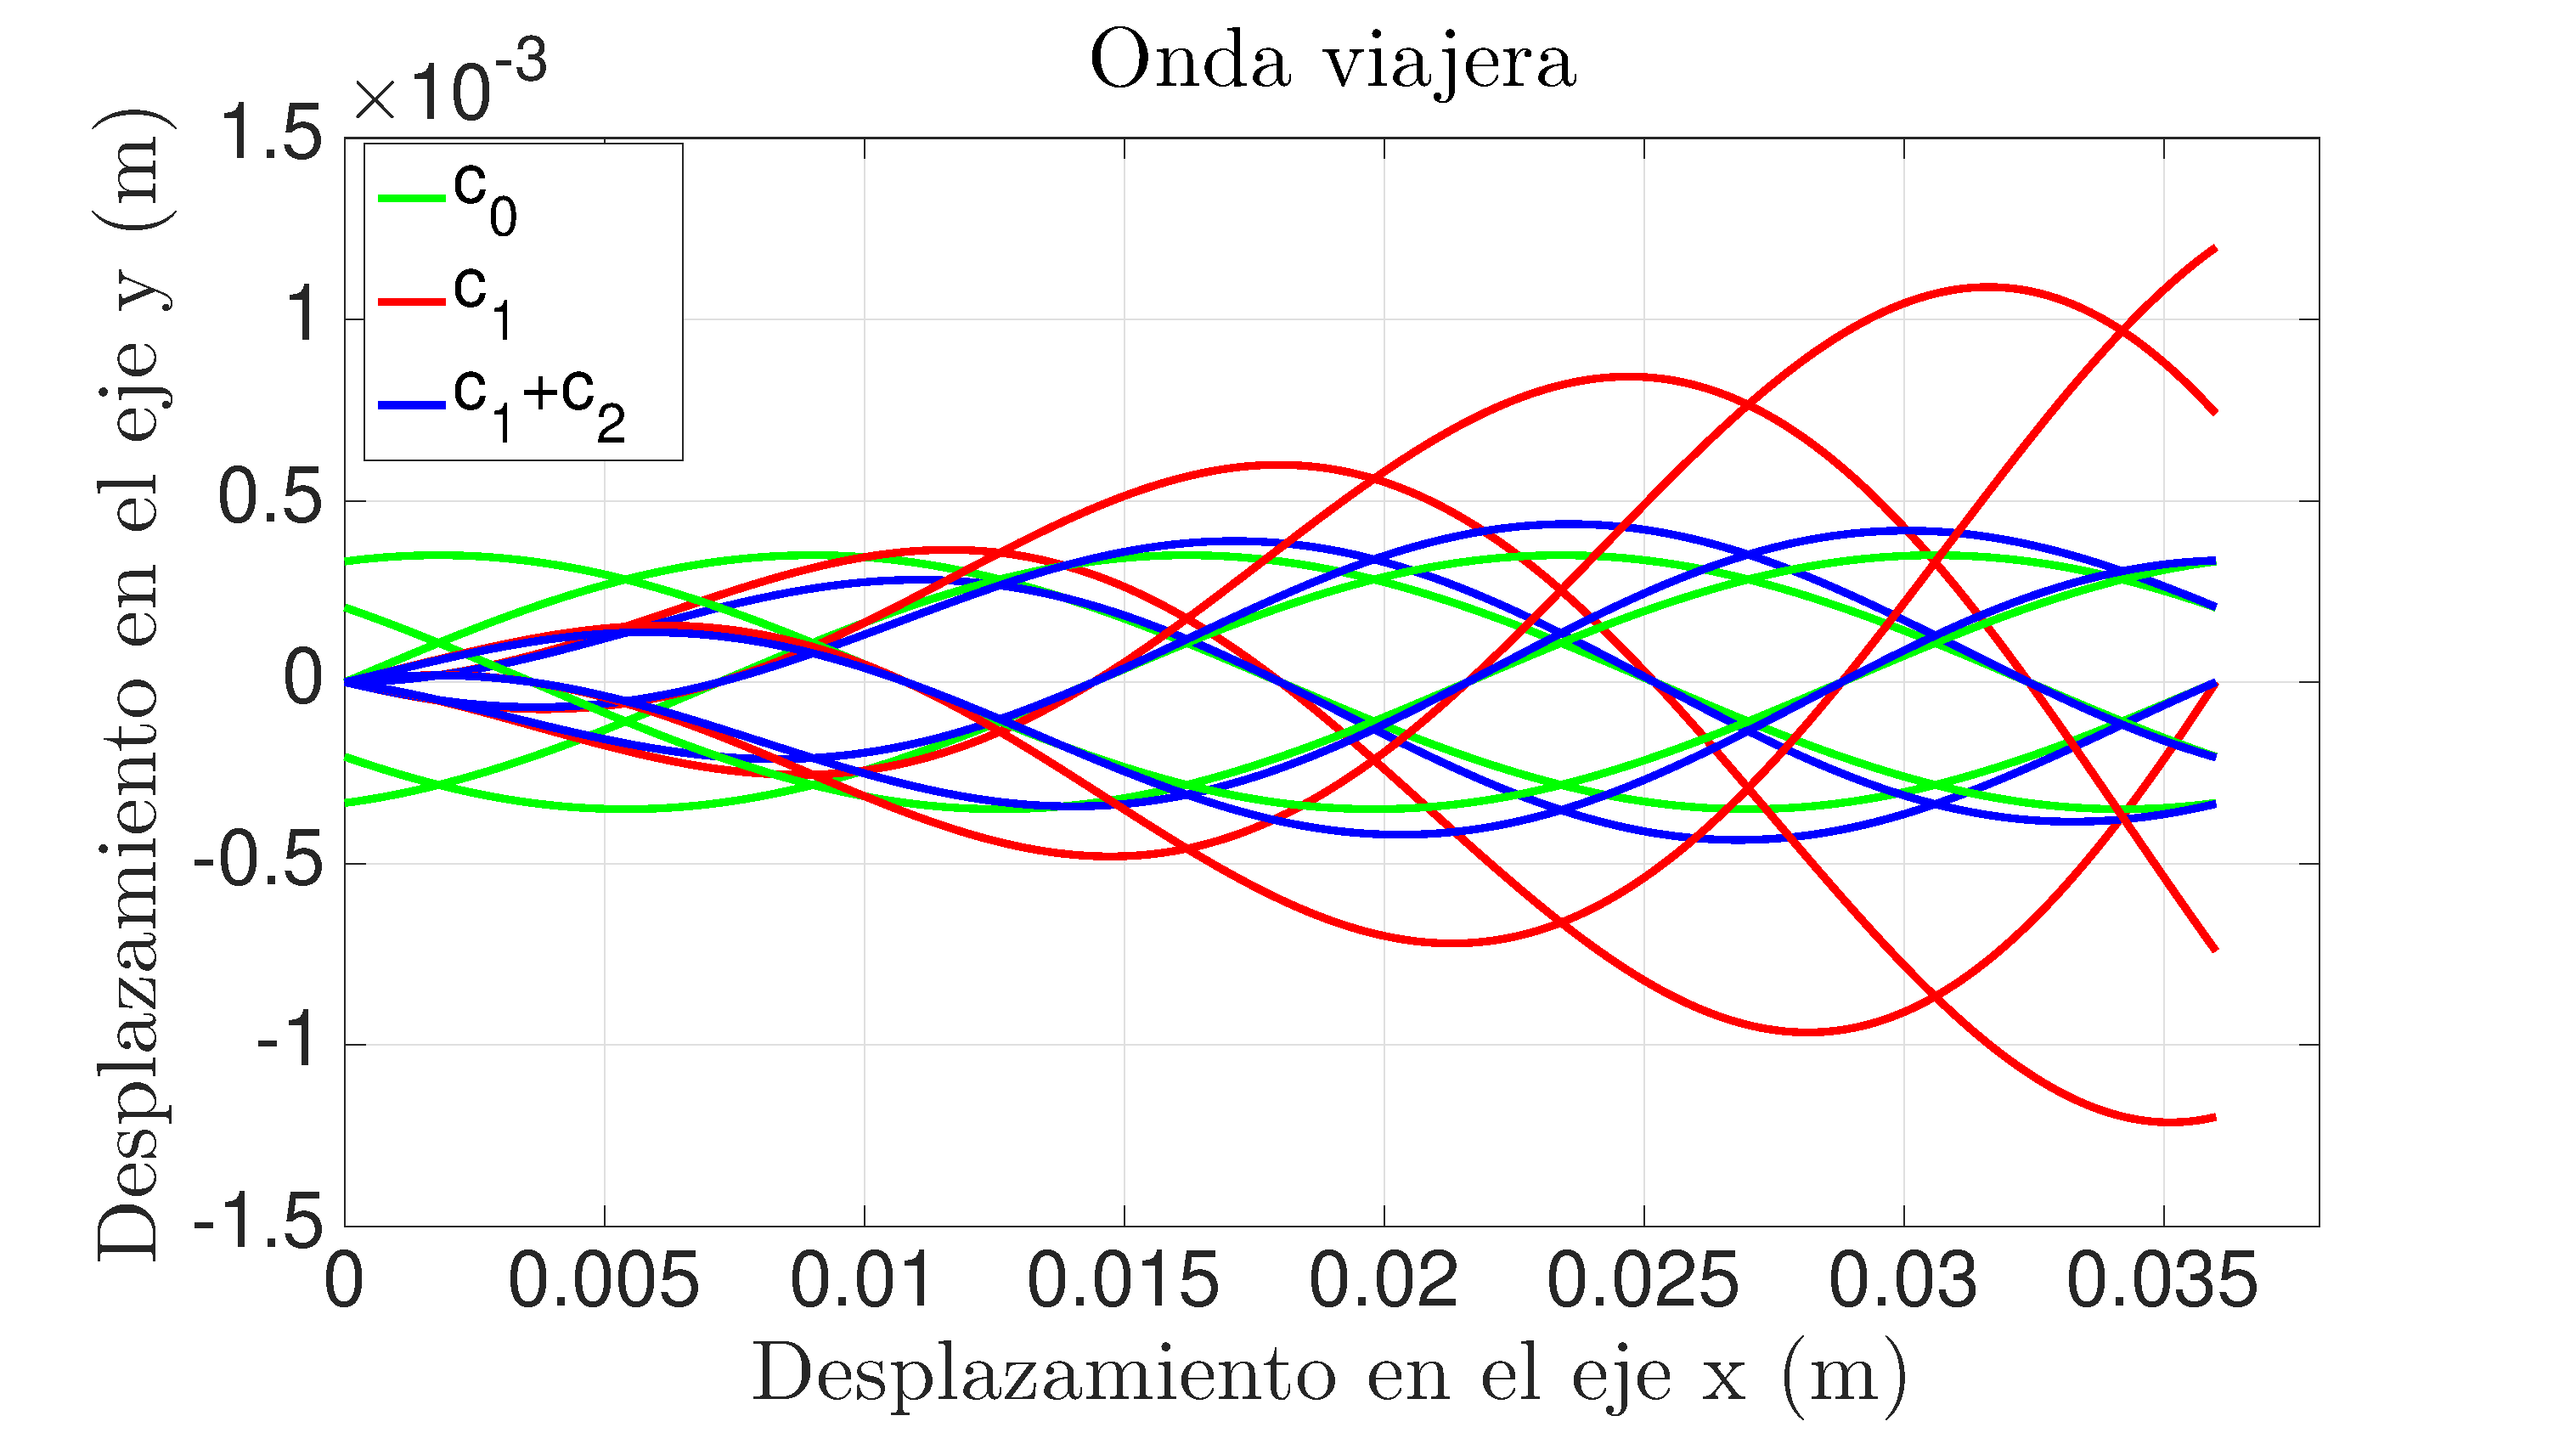
\includegraphics[width=0.43\textwidth]{Figuras/FC}
  	\caption{Comparación de la onda viajera para diferentes coeficientes.}
  	\label{fig:FC}
\end{figure}

Siguiendo el análisis descrito en \cite{gray1955propulsion}, se puede extraer la velocidad de avance para el movimiento indicado en (\ref{eq:flag_fish_traveling_wave}) como:
\begin{eqnarray}
\label{eq:Vx_fish}
\begin{split}
	V_x (t)  =  \pi f\left( \frac{C_N - C_L}{C_L} \right) \left( \frac{1}{ 1 + \frac{6 \pi R \mu}{n \lambda C_L} }  \right)\\
(- \frac{2 \pi}{\lambda} c_0^2 - 2 \pi c_0 c_1 - \frac{4 \pi c_0 c_2}{3} \\ 
+ c_0 c_1 \sin \left( 4 \pi f t \right) + c_0 c_2 \sin \left( 4 \pi f t \right) - \frac{2 \pi \lambda}{3} c_1^2 \\
- \pi \lambda^2 c_1 c_2 + \frac{\lambda c_1^2}{2} \sin \left( 4 \pi f t \right) + \lambda^2 c_1 c_2 \sin \left( 4 \pi f t \right) \\
- \frac{2 \pi \lambda^3}{5} c_2^2 + \frac{\lambda^3 c_2^2}{2} \sin \left( 4 \pi f t \right) )
	 		\end{split}
\end{eqnarray}
donde se aprecia la influencia de los coeficientes para lograr diferentes magnitudes de velocidad, y la relación entre ellos. Esto implica una cierta dificultad para alcanzar una velocidad óptima, y mantener un movimiento de onda viajera cuyas oscilaciones sean moduladas y mantenidas (constantes) en el espacio.\\

Para simplificar este cometido se opta por una descripción diferente del movimiento de onda viajera descrito en (\ref{eq:flag_fish_traveling_wave}), basado en un coeficiente fraccionario que influye en la amplitud de la onda viajera en base a su ubicación en el espacio, siendo por lo tanto la nueva expresión de la forma
\begin{eqnarray}
	\label{eq:flag_fish_traveling_wave_fractional}
	y (x,t) = c_1 x^{\alpha} \sin \left( \frac{2 \pi}{\lambda}  ( x - V_p t) \right).
\end{eqnarray}
\

Esta nueva descripción permite determinar la amplitud máxima de las oscilaciones a partir del coeficiente $c_1$, y modular su crecimiento con el parámetro $\alpha$. La Figura \ref{fig:OVF} evidencia este comportamiento, donde se puede observar el crecimiento en amplitud de la onda para diferentes valores del parámetro $\alpha$.
\begin{figure}[!h] %  figure placement: here, top, bottom, or page
	\vspace*{3mm}
    \centering
    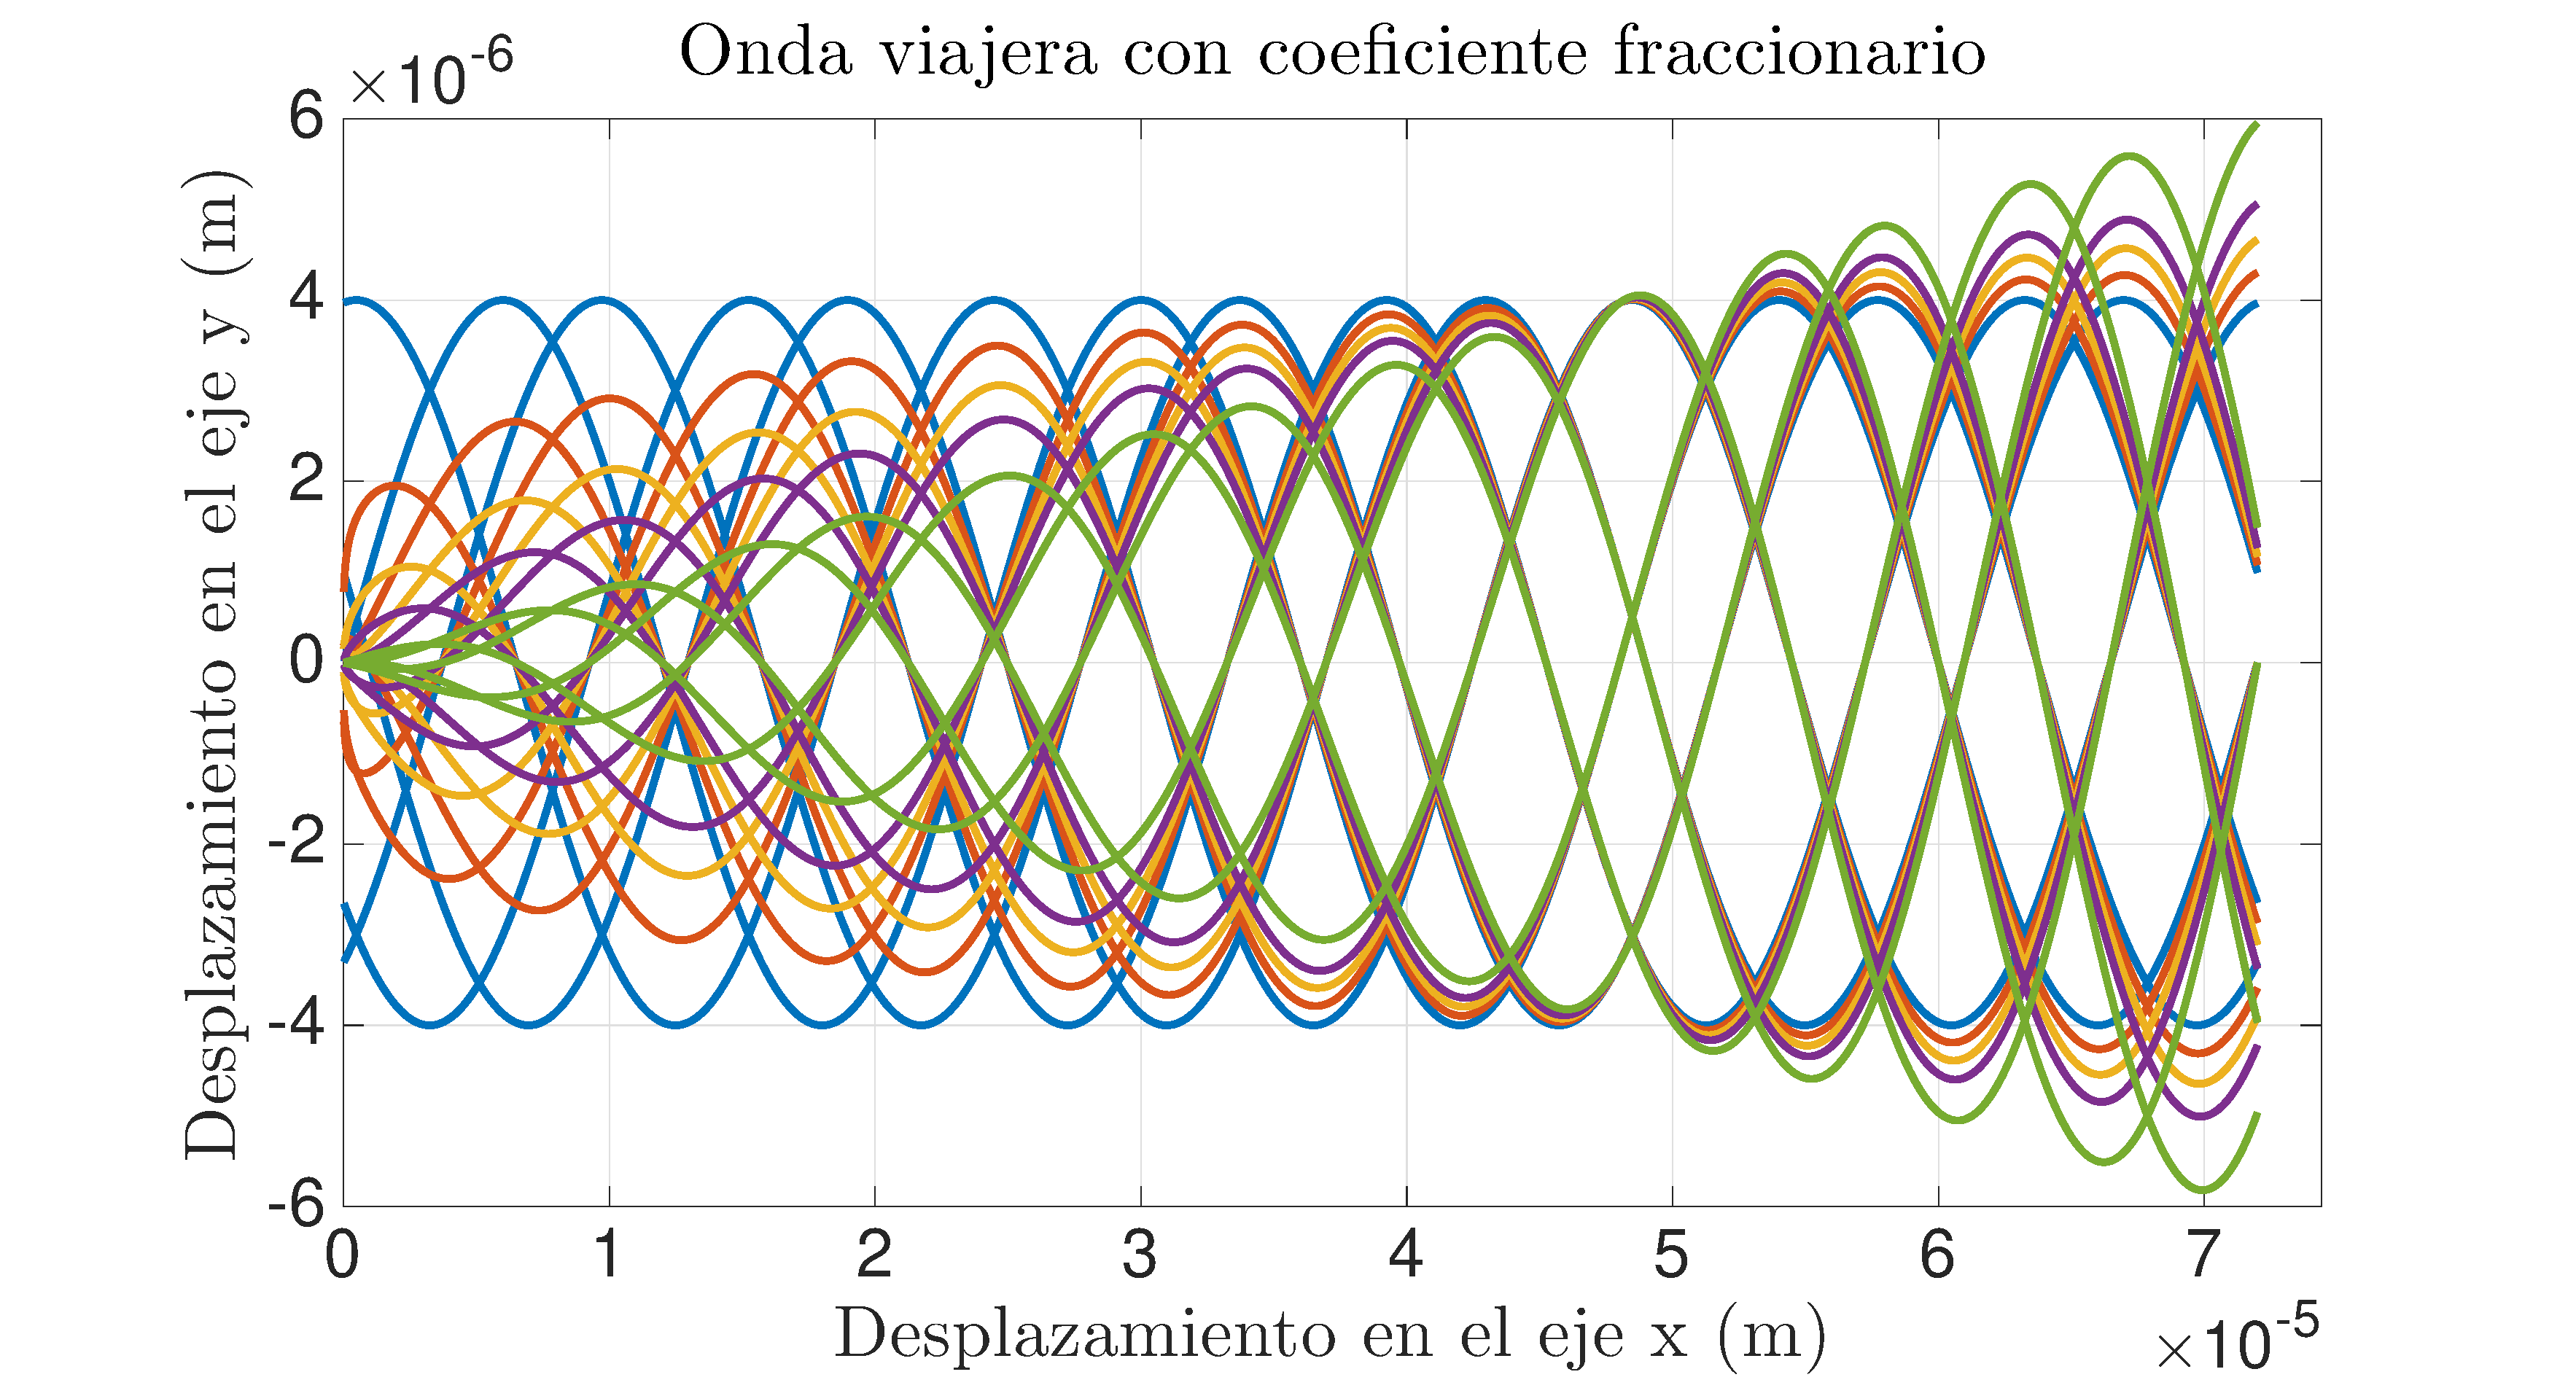
\includegraphics[width=0.6\textwidth]{Figuras/OVF}
  	\caption{Comparación de la onda viajera para diferentes coeficientes fraccionarios.}
  	\label{fig:OVF}
\end{figure}
 En esta representación el coeficiente $c_1$ es definido como $c_1 = \frac{A}{\lambda^{\alpha_0}}$, donde $A$ es la amplitud máxima de la oscilación, $\lambda$ la longitud del flagelo y $\alpha_0$ es $\alpha$, aunque valores próximos a este último permite modificar el crecimiento respecto a ese comportamiento fijo, pudiendo lograr crecimientos mas abrupto o suaves de las oscilaciones, si el valor es mayor o inferior respectivamente.\\
 
La onda de color azul representa el movimiento armónico de la onda viajera, mientras que las diferentes tonalidades, desde el color naranja hasta el verde representan el movimiento descrito para los valores de 0.2, 0.4, 0.6 y 1 de $\alpha$, respectivamente. Este barrido de valores de $\alpha$ permite determinar que valores cercanos a cero implican un crecimiento más rápido al inicio del flagelo y un crecimiento mas amortiguado una vez alcanzada la amplitud máxima deseada de las oscilaciones. Así mismo, valores próximos a la unidad implican un comportamiento completamente opuesto.\\

Mediante esta nueva expresión se consigue de definir un movimiento de onda viajera, cuyo crecimiento y modulación se encuentra regulado con un único parámetro. Además de proporcionar una velocidad mayor respecto al movimiento descrito en (\ref{eq:flag_fish_traveling_wave}) y por lo tanto más optima respecto al movimiento armónico de onda viajera. Aunque esta conclusión desea ser validada en este documento, en una primera instancia puede ser aceptada, pues a un 20.08\% de longitud del flagelo (10$^{-5}$ m ) el movimiento descrito por (\ref{eq:flag_fish_traveling_wave_fractional}) logra alcanzar una 73.12\% de la amplitud máxima deseada, frente al 21.06\% del movimiento representado por (\ref{eq:flag_fish_traveling_wave}).\\

Para justificar que este incremente de amplitud, se corresponde con un aumento de la fuerza de empuje y por lo tanto de la velocidad de avance, simplemente es necesario repetir el procedimiento que permitió calcular la velocidad de (\ref{eq:flag_fish_traveling_wave}) en (\ref{eq:Vx_fish}) \cite{gray1955propulsion}. Sin embargo, la integración del término exponencial de (\ref{eq:flag_fish_traveling_wave_fractional}) implica un proceso iterativo de resolución compleja. Inconveniente que pretende ser solventado mediante el uso de técnicas de integración numérica basado en una cuadratura adaptativa de Gauss-Kronrod.\\

A continuación se describe el procedimiento y software desarrollado para el calculado de la velocidad considerando oscilaciones de pequeña amplitud, donde los términos segundo orden son despreciados, y en una segunda perspectiva en la cual se tiene la influencia de dichos términos.





%---------------------------------------
% Capítulo 2: VELOCIDAD DE AVANCE DE ONDAS DE PEQUEÑA AMPLITUD
%---------------------------------------
% Resolución del problema a pequeñas dimensiones. Se desprecian los términos cuadráticos.
%---------------------------------------
\section{VELOCIDAD DE AVANCE DE ONDAS DE PEQUEÑA AMPLITUD} \label{sec:velocidad_pequena}
%---------------------------------------
Para cuantificar la velocidad de avance generada por el movimiento de onda viajera descrito, en primer lugar se describirán las ecuaciones diferenciales propuestas en \cite{Gray1955} para su cálculo. Posteriormente se verificará la precisión del método mediante las expresiones teóricas calculadas anteriormente y finalmente se determinará la velocidad para la nueva expresión de onda viajera propuesta (\ref{eq:flag_fish_traveling_wave_fractional}).
\begin{figure}[!h] %  figure placement: here, top, bottom, or page
	\vspace*{3mm}
    \centering
    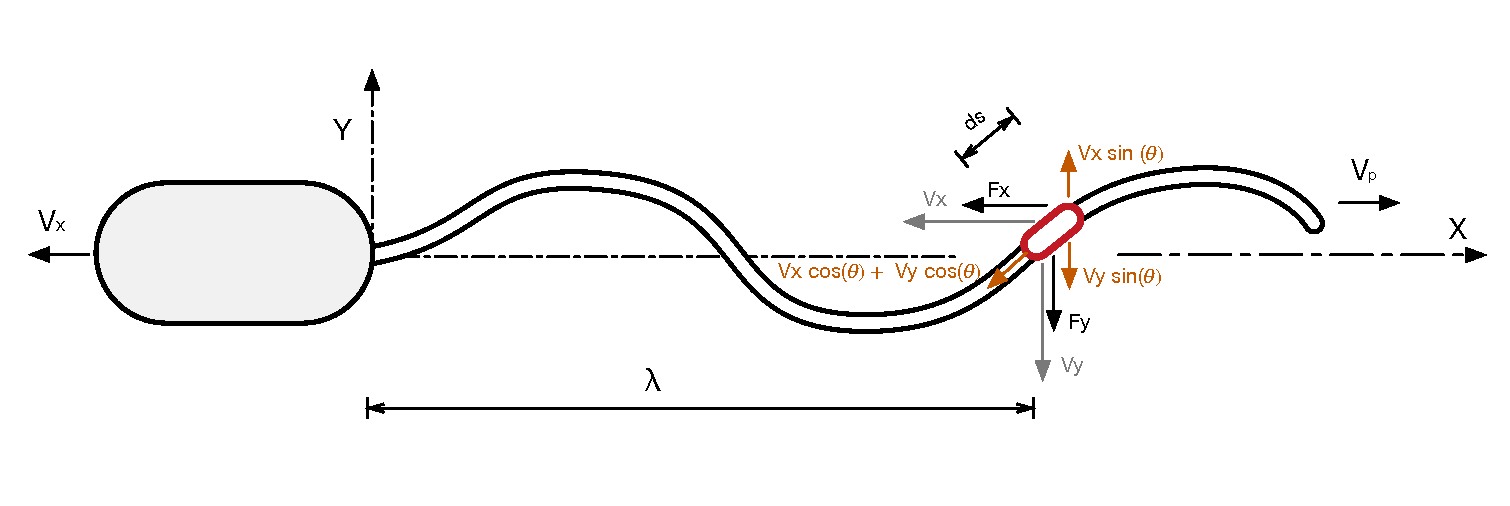
\includegraphics[width=0.9\textwidth]{Figuras/flagelo_dx}
  	\caption{Sólido libre de un elemento infinitesimal del flagelo.}
  	\label{fig:solido_flag}
\end{figure}

De acuerdo al planteamiento y análisis descrito en \cite{Gray1955} la velocidad lograda es debido a la fuerza de propulsión generada por el flagelo. Siendo la fuerza ejercida por un elemento infinitesimal del flagelo 
\begin{eqnarray}
	\label{eq:dF_ds}
	\frac{dF}{ds}= \frac{(C_N - C_L) \frac{dy}{dt}\frac{dy}{dx} - V_x \left(  C_L + C_N \frac{dy}{dx} ^2 \right)}{1 + \frac{dy}{dx}^2},
\end{eqnarray}
donde $y(x,t)$ define la forma de onda, $C_N$ y $C_L$ representan el coeficiente de rozamiento normal y tangencial, $V_x$ es la velocidad de avance, $\frac{dy}{dt}$ es la velocidad transversal y $\frac{dy}{dx}$ el ángulo de inclinación del elemento considerado respecto al eje de desplazamiento. Suponiendo unas dimensiones y oscilaciones relativamente pequeñas, es posible aproximar el diferencial de superficie por un diferencial de longitud ($ds \approx dx$) y despreciar los términos de segundo orden. Así pues, es posible conocer la velocidad de avance afirmando que la fuerza de propulsión total para una oscilación completa es igual a la fuerza necesaria para vencer la fuerza de arrastre debida al cuerpo, descrita como:
\begin{eqnarray}
	\label{eq:dF=}
	nF = C_C V_x
\end{eqnarray}
donde $n$ es el número oscilaciones simultáneas que recorren el flagelo y $C_C$ representa el coeficiente de arrastre de la cabeza, que para una esfera de radio $R$ viene dado por la expresión
\begin{equation}
C_C=6 \pi \mu R.
\end{equation}
\

Respecto las derivadas respecto del tiempo y el espacio de las ecuaciones definidas anteriormente (\ref{eq:flag_fish_traveling_wave}) y (\ref{eq:flag_fish_traveling_wave_fractional}) son:
\begin{eqnarray}
	\label{eq:dy_dt}
	\frac{dy}{dt} = - \frac{2 \pi V_p}{\lambda}  (c_0 + c_1 x^{\alpha} + c_2 x^2) \cos \left( \frac{2 \pi}{\lambda}  ( x - V_p t) \right), 
\end{eqnarray}
\begin{eqnarray}
	\label{eq:dy_dx}
		\frac{dy}{dx} = \frac{2 \pi }{\lambda}  (c_0 + c_1 x^{\alpha} + c_2 x^2) \cos \left( \frac{2 \pi}{\lambda}  ( x - V_p t) \right)\\
		 + (\alpha c_1 x^{\alpha-1} + 2 c_2 x) \sin \left(  \frac{2 \pi}{\lambda}  ( x - V_p t) \right), \nonumber
\end{eqnarray}

términos que representan la principal complejidad para su integración numérica y algebraica. Además de ser los principales componentes que determinan la fuerza de propulsión.\\

Después de varias cálculos y simplificaciones, es posible presentar la velocidad de avance como la siguiente ecuación diferencial:
\begin{eqnarray}
\label{eq:Vx_dx}
	\frac{V_x (t)}{dx} =  \left( \frac{C_N - C_L}{C_L} \right) \left( \frac{1}{ n \lambda + \frac{6 \pi R \mu}{C_L} }  \right) \frac{dy}{dt} \frac{dy}{dx}.
	\end{eqnarray}

%---------------------------------------
\subsection{Descripción del script de integración numérica} \label{sec:descripcion_script}
%-------------------------------------
Para implementar el script de integración numérica la ecuación anterior han sido agrupada en diversos términos como se muestra en la siguiente Figura:
\begin{figure}[!h] %  figure placement: here, top, bottom, or page
	\vspace*{3mm}
    \centering
    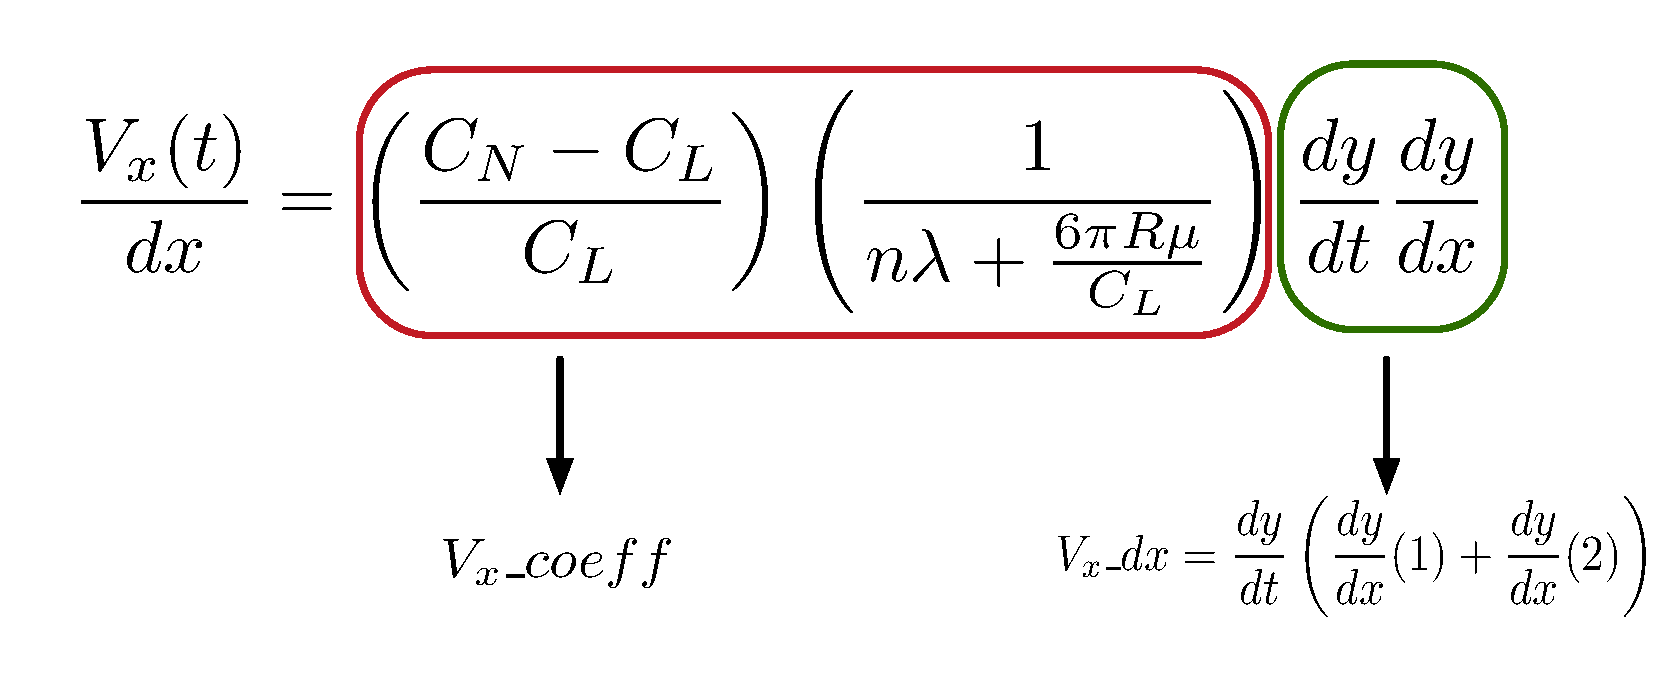
\includegraphics[width=0.6\textwidth]{Figuras/FDF}
  	\caption{Agrupación de términos.}
  	\label{fig:OVF}
\end{figure}

donde $V_{x}\_coeff$ es un término constante, y $V_x\_dx$ representa el producto de las derivadas indicadas anteriormente (\ref{eq:dy_dt}) y (\ref{eq:dy_dx}), las cuales son dependientes del tiempo y el espacio. Además, la derivada respecto al espacio ha sido separada en sus dos sumandos principales para una mejor compresión del código desarrollado.\\

Respecto a las funciones diferenciales han sido definidas como funciones paramétricas dependientes de la coordenada en el espacio, para cada instante de tiempo. Siendo necesario un bucle de interacción que calcule la velocidad de avance en cada instante de tiempo, obteniendo así un array de velocidades. A continuación se muestra el fragmento del script donde se obtiene el valor de la velocidad.
\begin{lstlisting}[]
%% Calculo de la velocidad de avance por integración numérica.

% Vx = (n * (CN - CL)) / (Cc + n * lambda * CL) * ( dy / dt * dy/dx dx)
% Vx = |------------- vx_coeff ---------------| * |------ vx_dx -------|
%                                         |-- dy_dt * (dy_dx1 + dy_dx2) --|

vx_coeff = ( (1/lambda) * (CN - CL) / CL )...
            * ( 1 / (1 + Cc/ ( n * lambda * CL) ) ) ;

for i=1:length(t);
  
    dy_dt =@(x) -(2*pi*Vp/lambda) * (c0 + c1.*x.^alfa  + c2.*x.^2)...
                .* cos( (2*pi/lambda) * (x - Vp*t(i)) );

    dy_dx1 =@(x) (2*pi/lambda) .* (c0 + c1.*x.^alfa + c2.*x.^2)...
                .* cos( (2*pi/lambda) * (x - Vp.*t(i)) );
    
    dy_dx2 =@(x) (2*c2.*x + alfa.*c1.*x.^(alfa-1))...
                .* sin( (2*pi/lambda) * (x - Vp.*t(i)) ); 
        
    vx_dx =@(x) dy_dt(x) .* (dy_dx1(x) + dy_dx2(x));                                     
   	
   	% Función de integración numérica -- quadgk
    % Numerically evaluate integral, adaptive Gauss-Kronrod quadrature.
    NVx = [NVx  quadgk(vx_dx,0,lambda)];
end
                                
NVx = NVx .* vx_coeff;

\end{lstlisting}
\

La función utilizada para realizar concretamente la integración numérica es la indicada en el extracto anterior del script ``\textbf{quadgk}''. Función que emplea un algoritmo de cálculo basado en la cuadratura adaptativa de Gauss-Kronrod. Respecto a su parámetros de configuración se han utilizados los definidos por defecto, es decir, una tolerancia absoluta de $10^{-10}$ y relativa de $10^{-6}$ para variables de tipo \textit{double}.

%---------------------------------------
\subsection{Verificación y validación del algoritmo de integración numérica} \label{sec:verificacion_script}
%-------------------------------------

Una vez desarrollado el script el siguiente paso es verificar que los resultados ofrecidos por la función de cálculo numérico son válidos en comparación a valores conocido. Por ello, en primer lugar se calculara la velocidad para la expresión de onda viajera (\ref{eq:flag_fish_traveling_wave}), cuya velocidad teórica conocida a través de (\ref{eq:Vx_fish}). Aunque previamente es necesario indicar cuales serán el valor numérico de los parámetros que serán usados, los cuales se exponen en la Tabla \ref{Tab:data_flagellum}.\\
\begin{table}[!h]
\centering
\caption{Valor de los parámetros, extraídos de \cite{Gray1955}}
\resizebox{0.9\textwidth}{!}{
\begin{tabular}{| c | c | c |}
  \hline
\cellcolor{lightgray} \textbf{Parámetros} & \cellcolor{lightgray} 
 \textbf{Expresión/Valor} & \cellcolor{lightgray} \textbf{Descripción} \\
 	\hline
$c_0$		& $4 \cdot 10^{-6}$ (m) & Amplitud máxima de las ondas. \\	
	\hline
$f$		& 35 (Hz) & Frecuencia de propagación.\\	
	\hline	
$\lambda$ & $24 \cdot 10^{-6}$  (m) & Longitud de onda de la onda viajera.	\\
	\hline
$n$ & $3$ & Numero de ondas simultáneas en el flagelo.	\\
	\hline
$R$ &  $5 \cdot 10^{-7}$ (m) & Radio de la cabeza. \\
	\hline
$d$ & $ 2 \cdot 10^{-7}$ (m)  & Radio del flagelo. \\
	\hline
$C_L$	& $\frac{2 \pi \mu }{ \log{\frac{d}{2 \lambda}} + \frac{1}{2}}$ & Coeficiente de arrastre tangencial. \\
	\hline
$C_N$	& $C_N = 2 C_L$ & Coeficiente de arrastre normal.\\
	\hline	
$C_C$	& 6$\pi$$\mu$$R$ & Coeficiente de arrastre de la cabeza.\\
  \hline
$\mu$ & $7^{-4}$ (Pa $\cdot$ s) & Viscosidad	 \cite{Majumdar2009}.	\\
	\hline		
\end{tabular}
\label{Tab:data_flagellum}
}
\end{table}

Una vez conocidos los datos, es posible verificar los resultados teóricos y numéricos obtenidos para diferentes magnitudes de los coeficientes de amplitud. Dichos coeficientes han sido seleccionados de forma que permitan alcanzar la amplitud máxima al final de una longitud de onda del flagelo, como se puede observar en la Figura \ref{fig:OVV}, donde el color azul representa la onda armónica, el verde la onda viajera de crecimiento lineal, y el color rojo identifica la onda viajera cuyo crecimiento es modulado con el coeficiente $c_2$.\\
\begin{figure}[!h] %  figure placement: here, top, bottom, or page
	\vspace*{3mm}
    \centering
    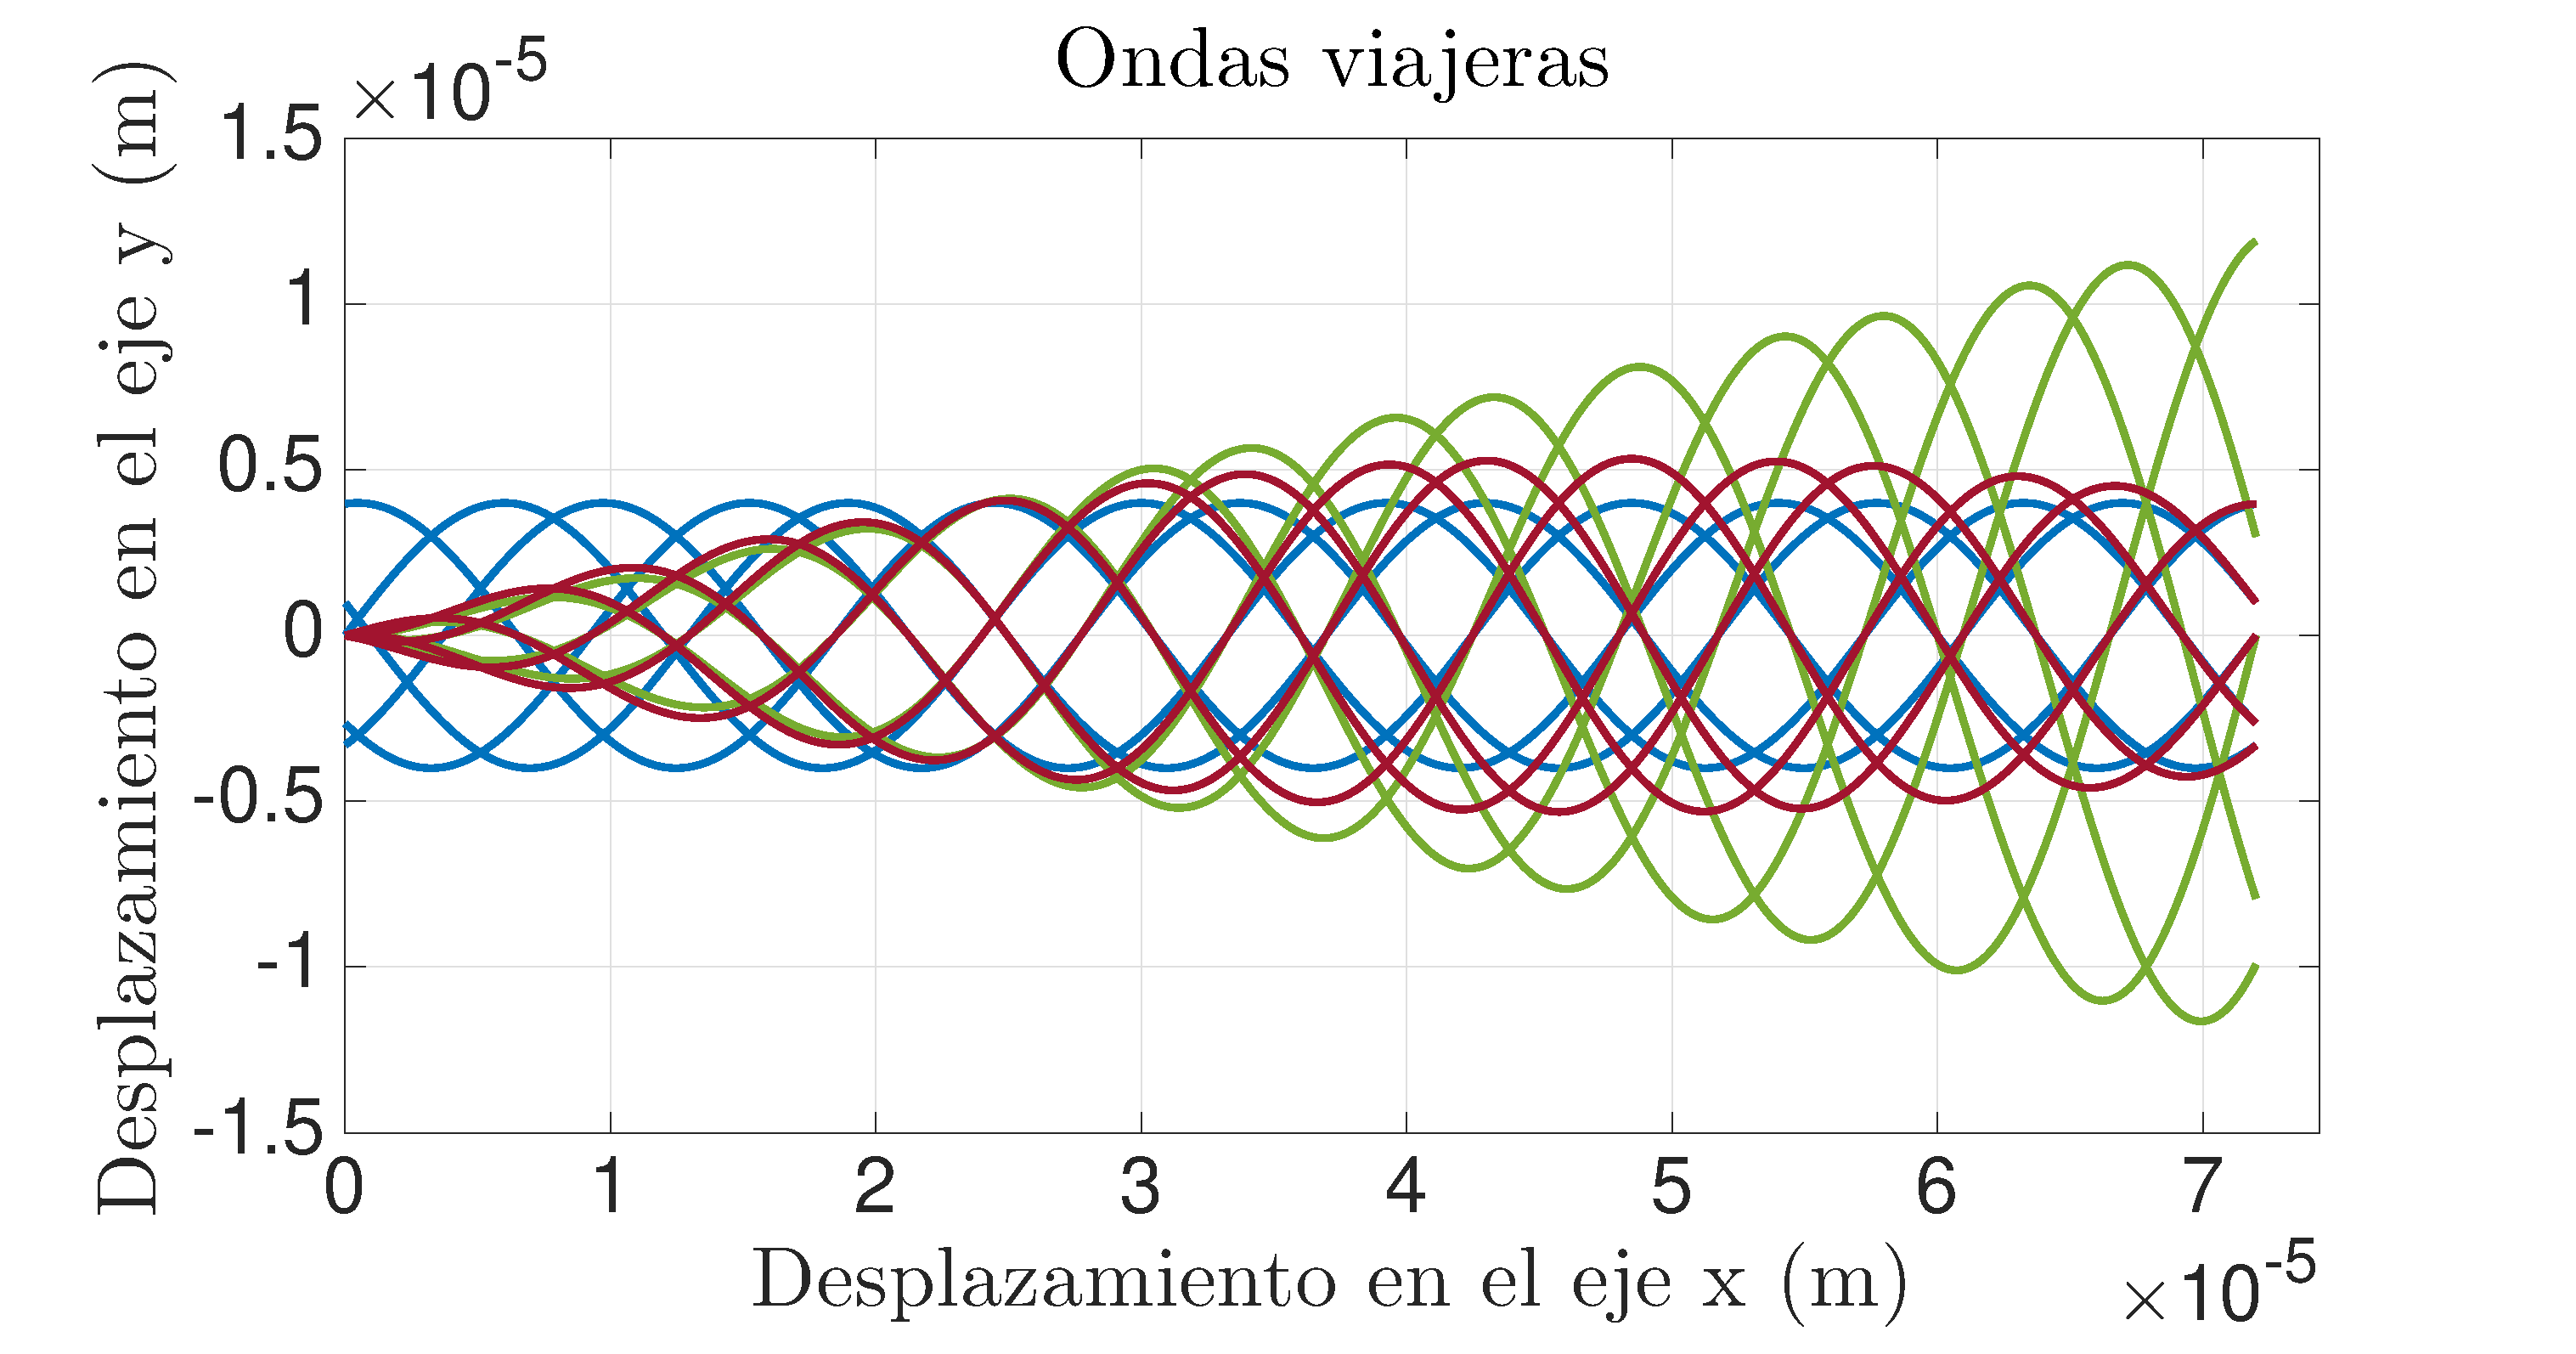
\includegraphics[width=0.9\textwidth]{Figuras/OVV}
  	\caption{Representación de las ondas viajeras empleadas para la verificación.}
  	\label{fig:OVV}
\end{figure}

De acuerdo al criterio de crecimiento en una longitud de onda el coeficiente $c_1$ se encuentran definido para la siguiente expresión
\begin{eqnarray}
	\label{eq:coeff_c1}
	c_1 = \frac{c_0}{n\lambda}.
\end{eqnarray}

Por otro lado, la combinación de los coeficientes $c_1$ y $c_2$ son definidos por (\ref{eq:coeff_c1yc2}), donde $m$ es un múltiplo de $\lambda$ y cumple la condición $m > n$.
\begin{eqnarray}
	\label{eq:coeff_c1yc2}
	c_1 &=& \frac{c_0 }{n \lambda} + \frac{m}{m - n}  \left( \frac{c_0} {m  \lambda} - \frac{n A} {m  \lambda} \right)\\
	c_2 &=& \frac{m}{m - n}  \left( \frac{A} {m  \lambda^2} - \frac{c_0} {n m  \lambda^2} \right) \nonumber
\end{eqnarray}

Finalmente los resultados obtenidos se muestran en la Figura \ref{fig:OVV}, lo cuales aprueban la validez del algoritmo y la función para calcular la velocidad de avance del movimiento de onda viajera por integración numérica. En dichos resultados se puede observar que tanto el valor obtenido por la función teórica (\ref{eq:Vx_fish}) e integración numérica coinciden con un RMSE de $ 2 \cdot 10^{-19}$ \% aproximadamente.
\begin{figure}[t] %  figure placement: here, top, bottom, or page
	\vspace*{3mm}
    \centering
    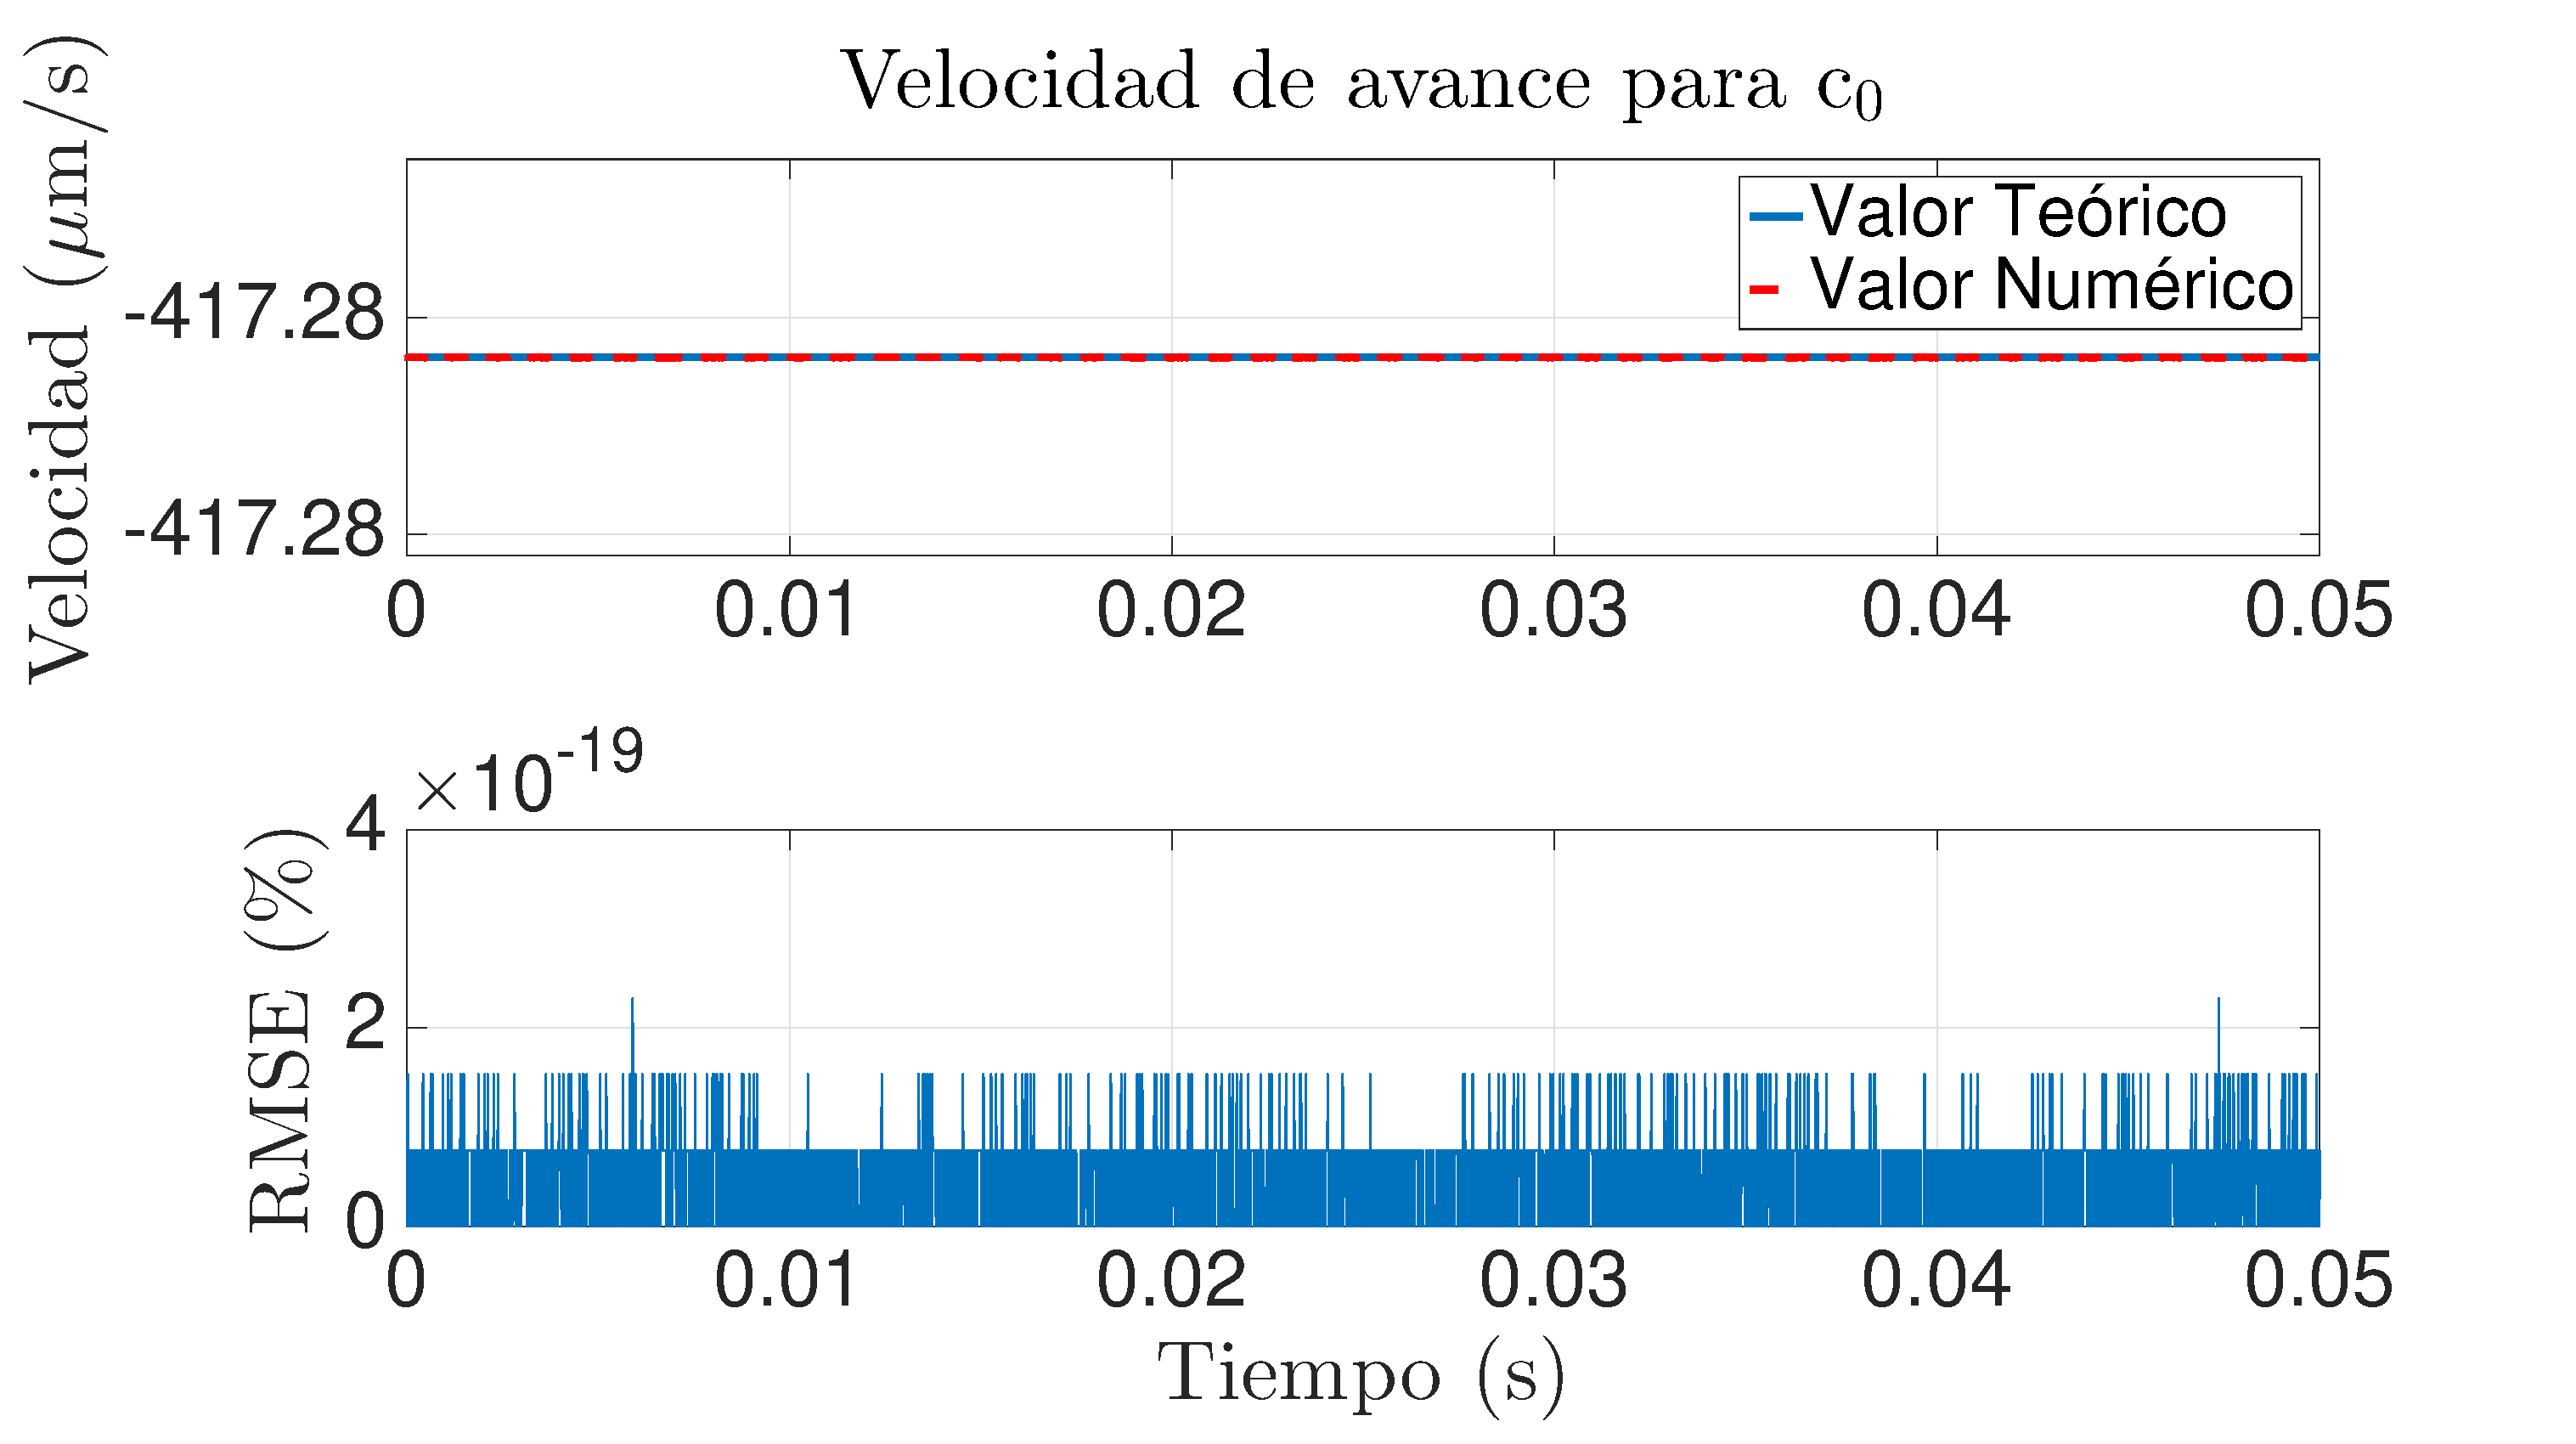
\includegraphics[width=0.45\textwidth]{Figuras/VC0}
    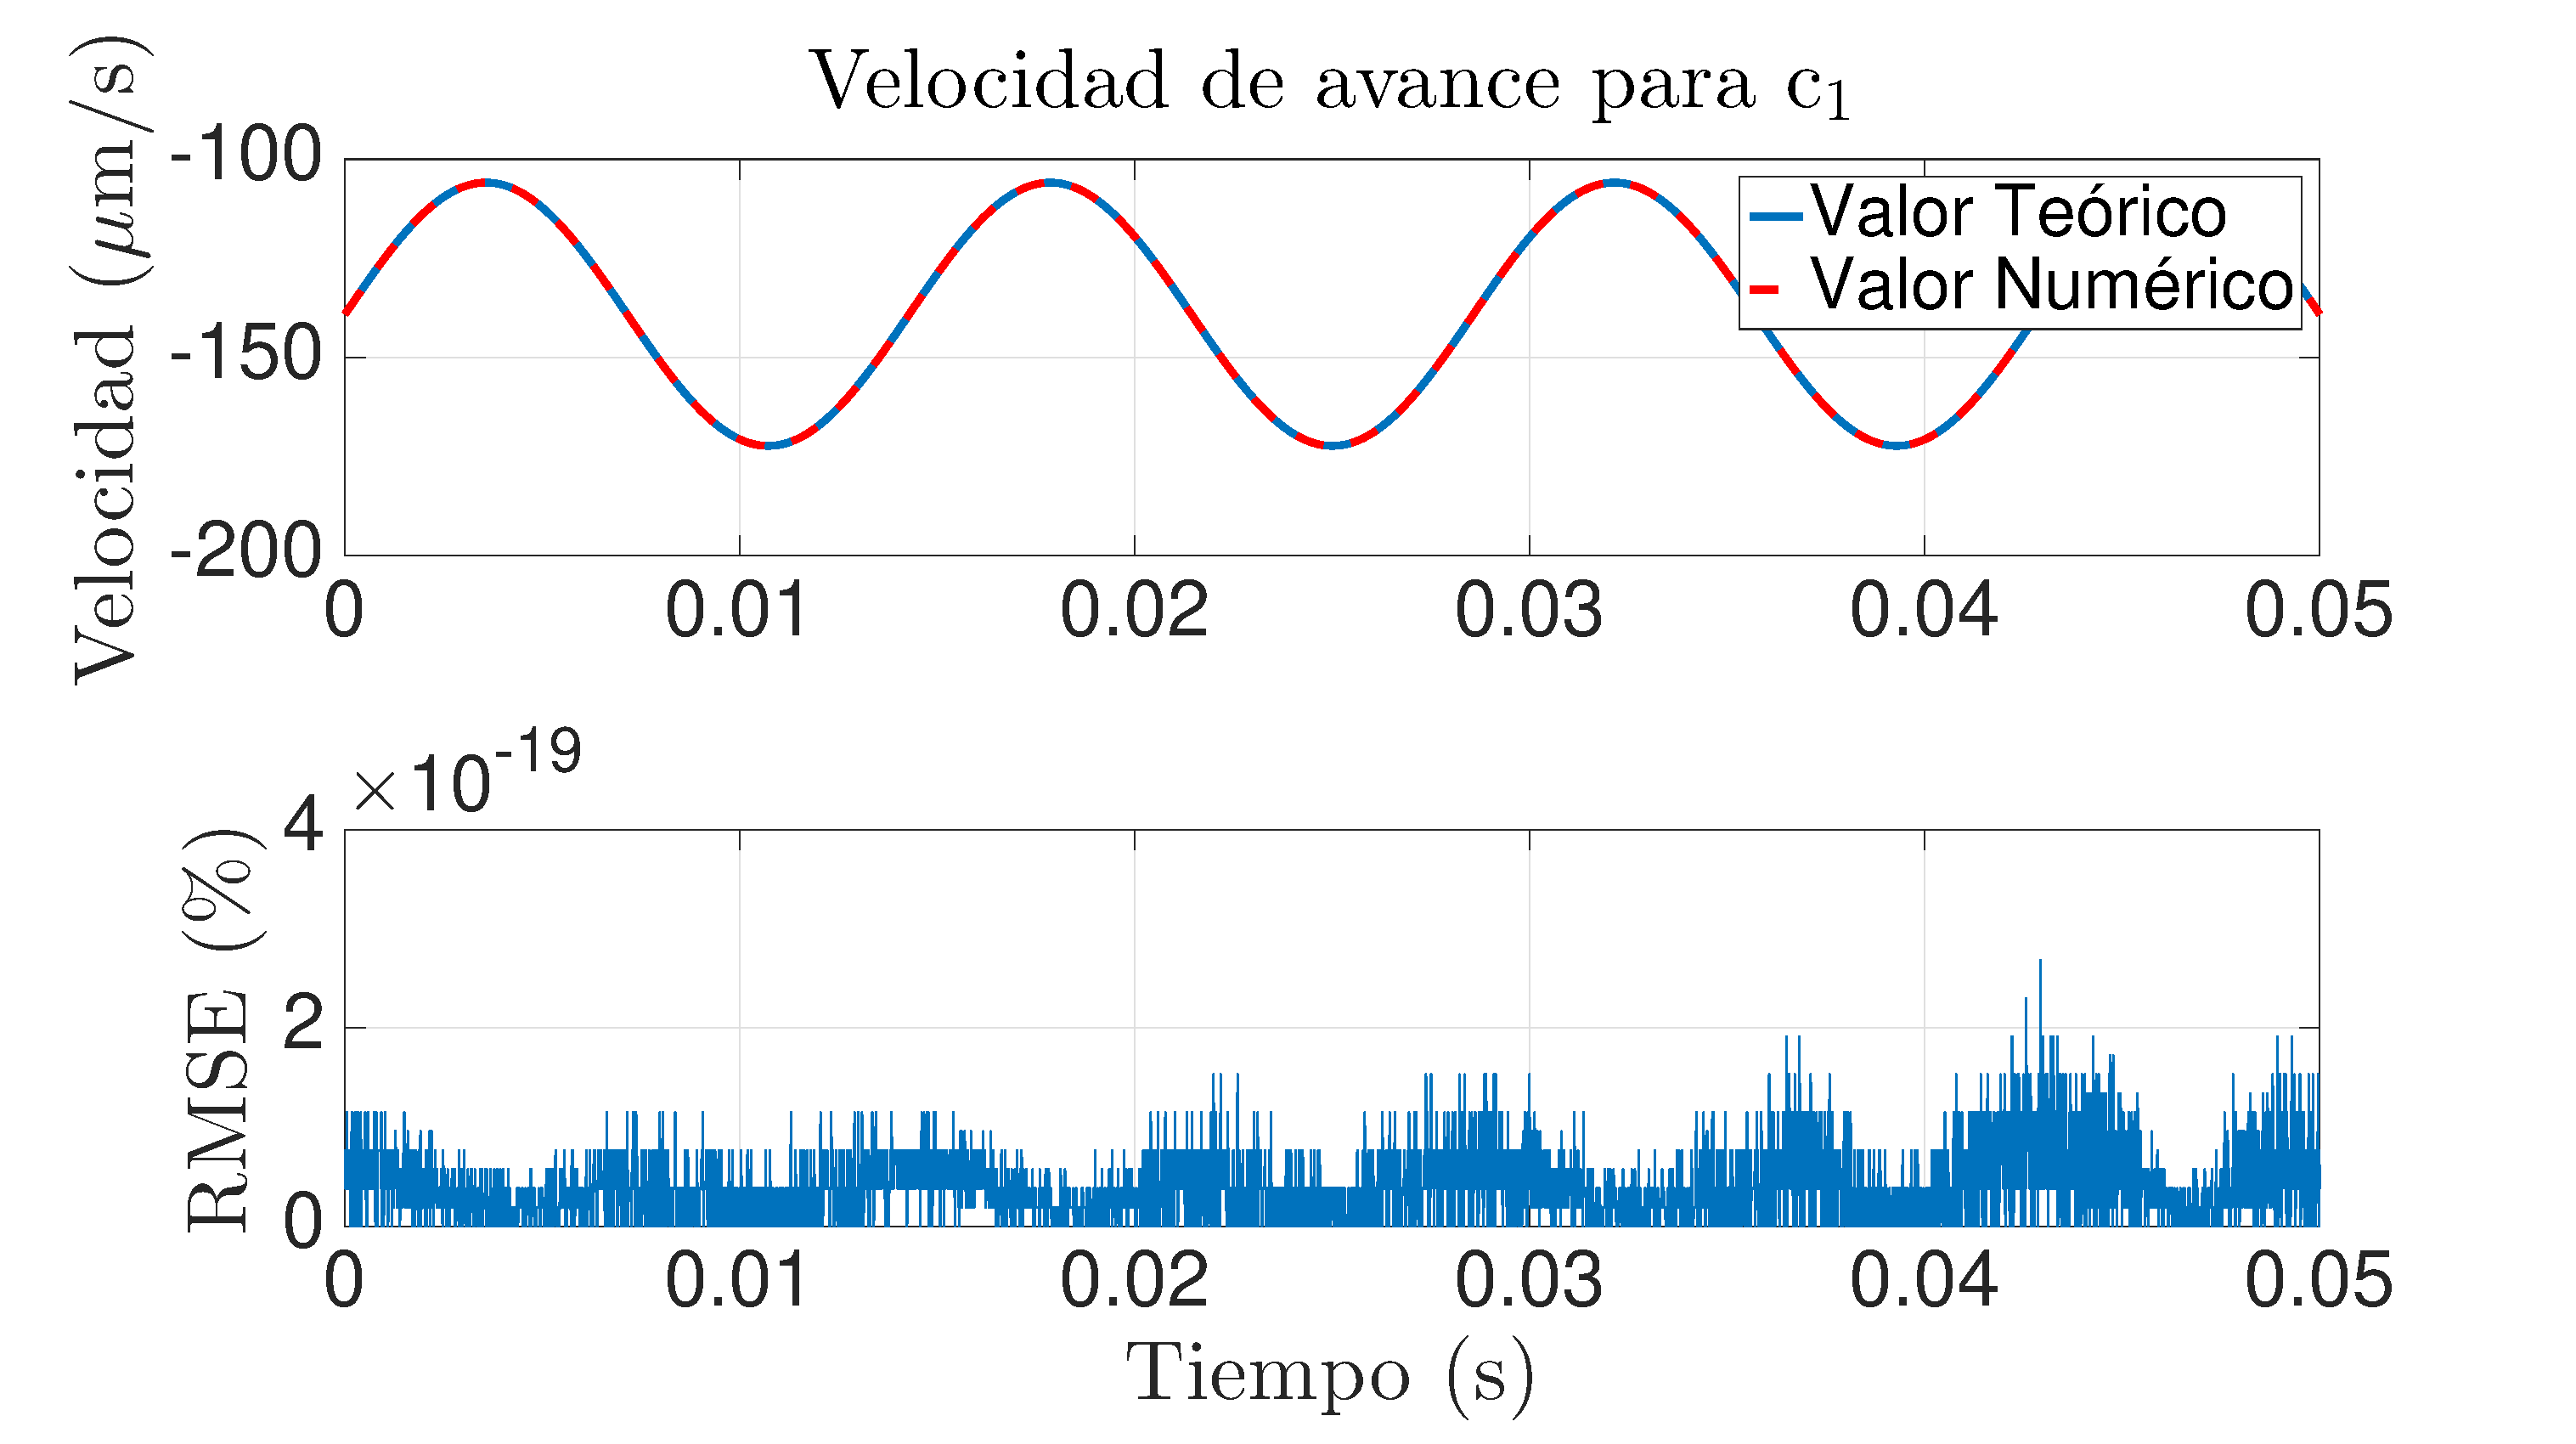
\includegraphics[width=0.45\textwidth]{Figuras/VC1}
    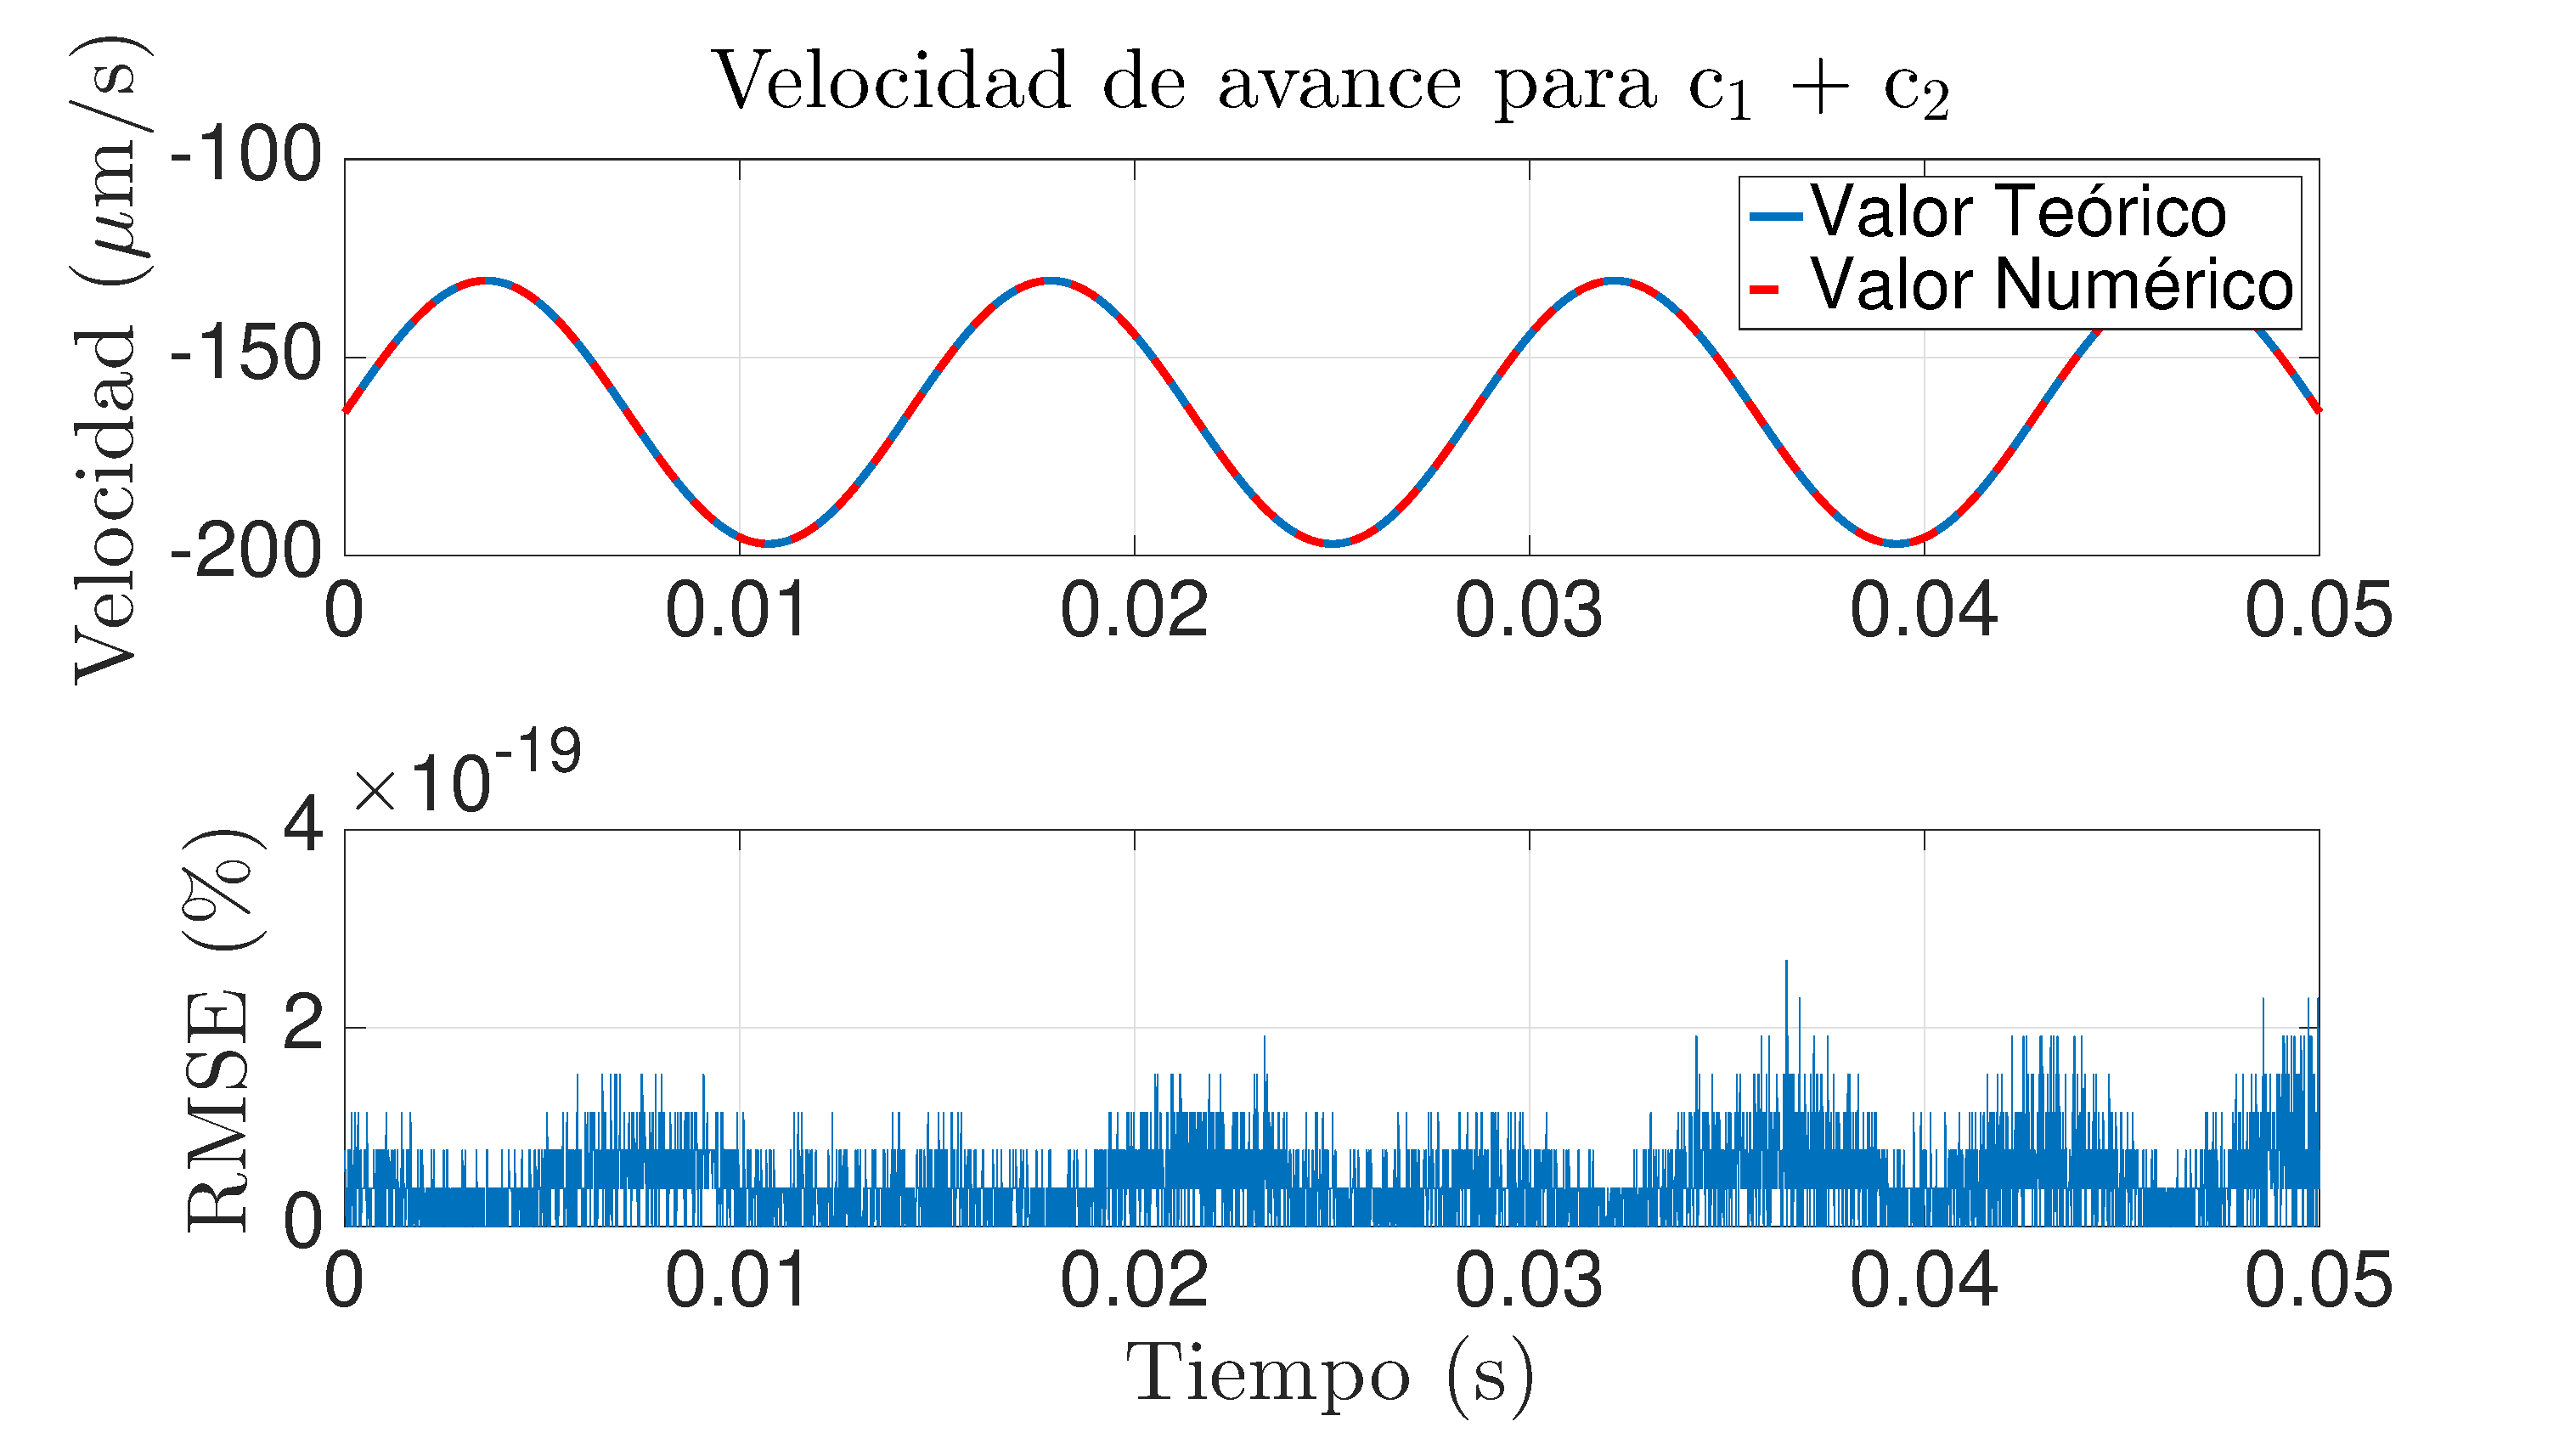
\includegraphics[width=0.5\textwidth]{Figuras/VC2}
  	\caption{Verificación algoritmo de integración numérica.}
  	\label{fig:OVVC}
\end{figure}
\newpage
%---------------------------------------
\subsection{Cálculo y análisis de velocidad de onda viajera fraccionaria} \label{sec:analisis_velocidad}
%-------------------------------------

Después de verificar que el script desarrollado es válido, proporcionando unos datos coherentes respecto a los valores teóricos. Se va a analizar la velocidad obtenida para la expresión de onda viajera indicada en (\ref{eq:flag_fish_traveling_wave_fractional}) y representadas en la Figura \ref{fig:OVF}. Siendo sus respectivas velocidades las mostradas en la Figura \ref{fig:VCF}. 
\begin{figure}[!h] %  figure placement: here, top, bottom, or page
	\vspace*{3mm}
    \centering
    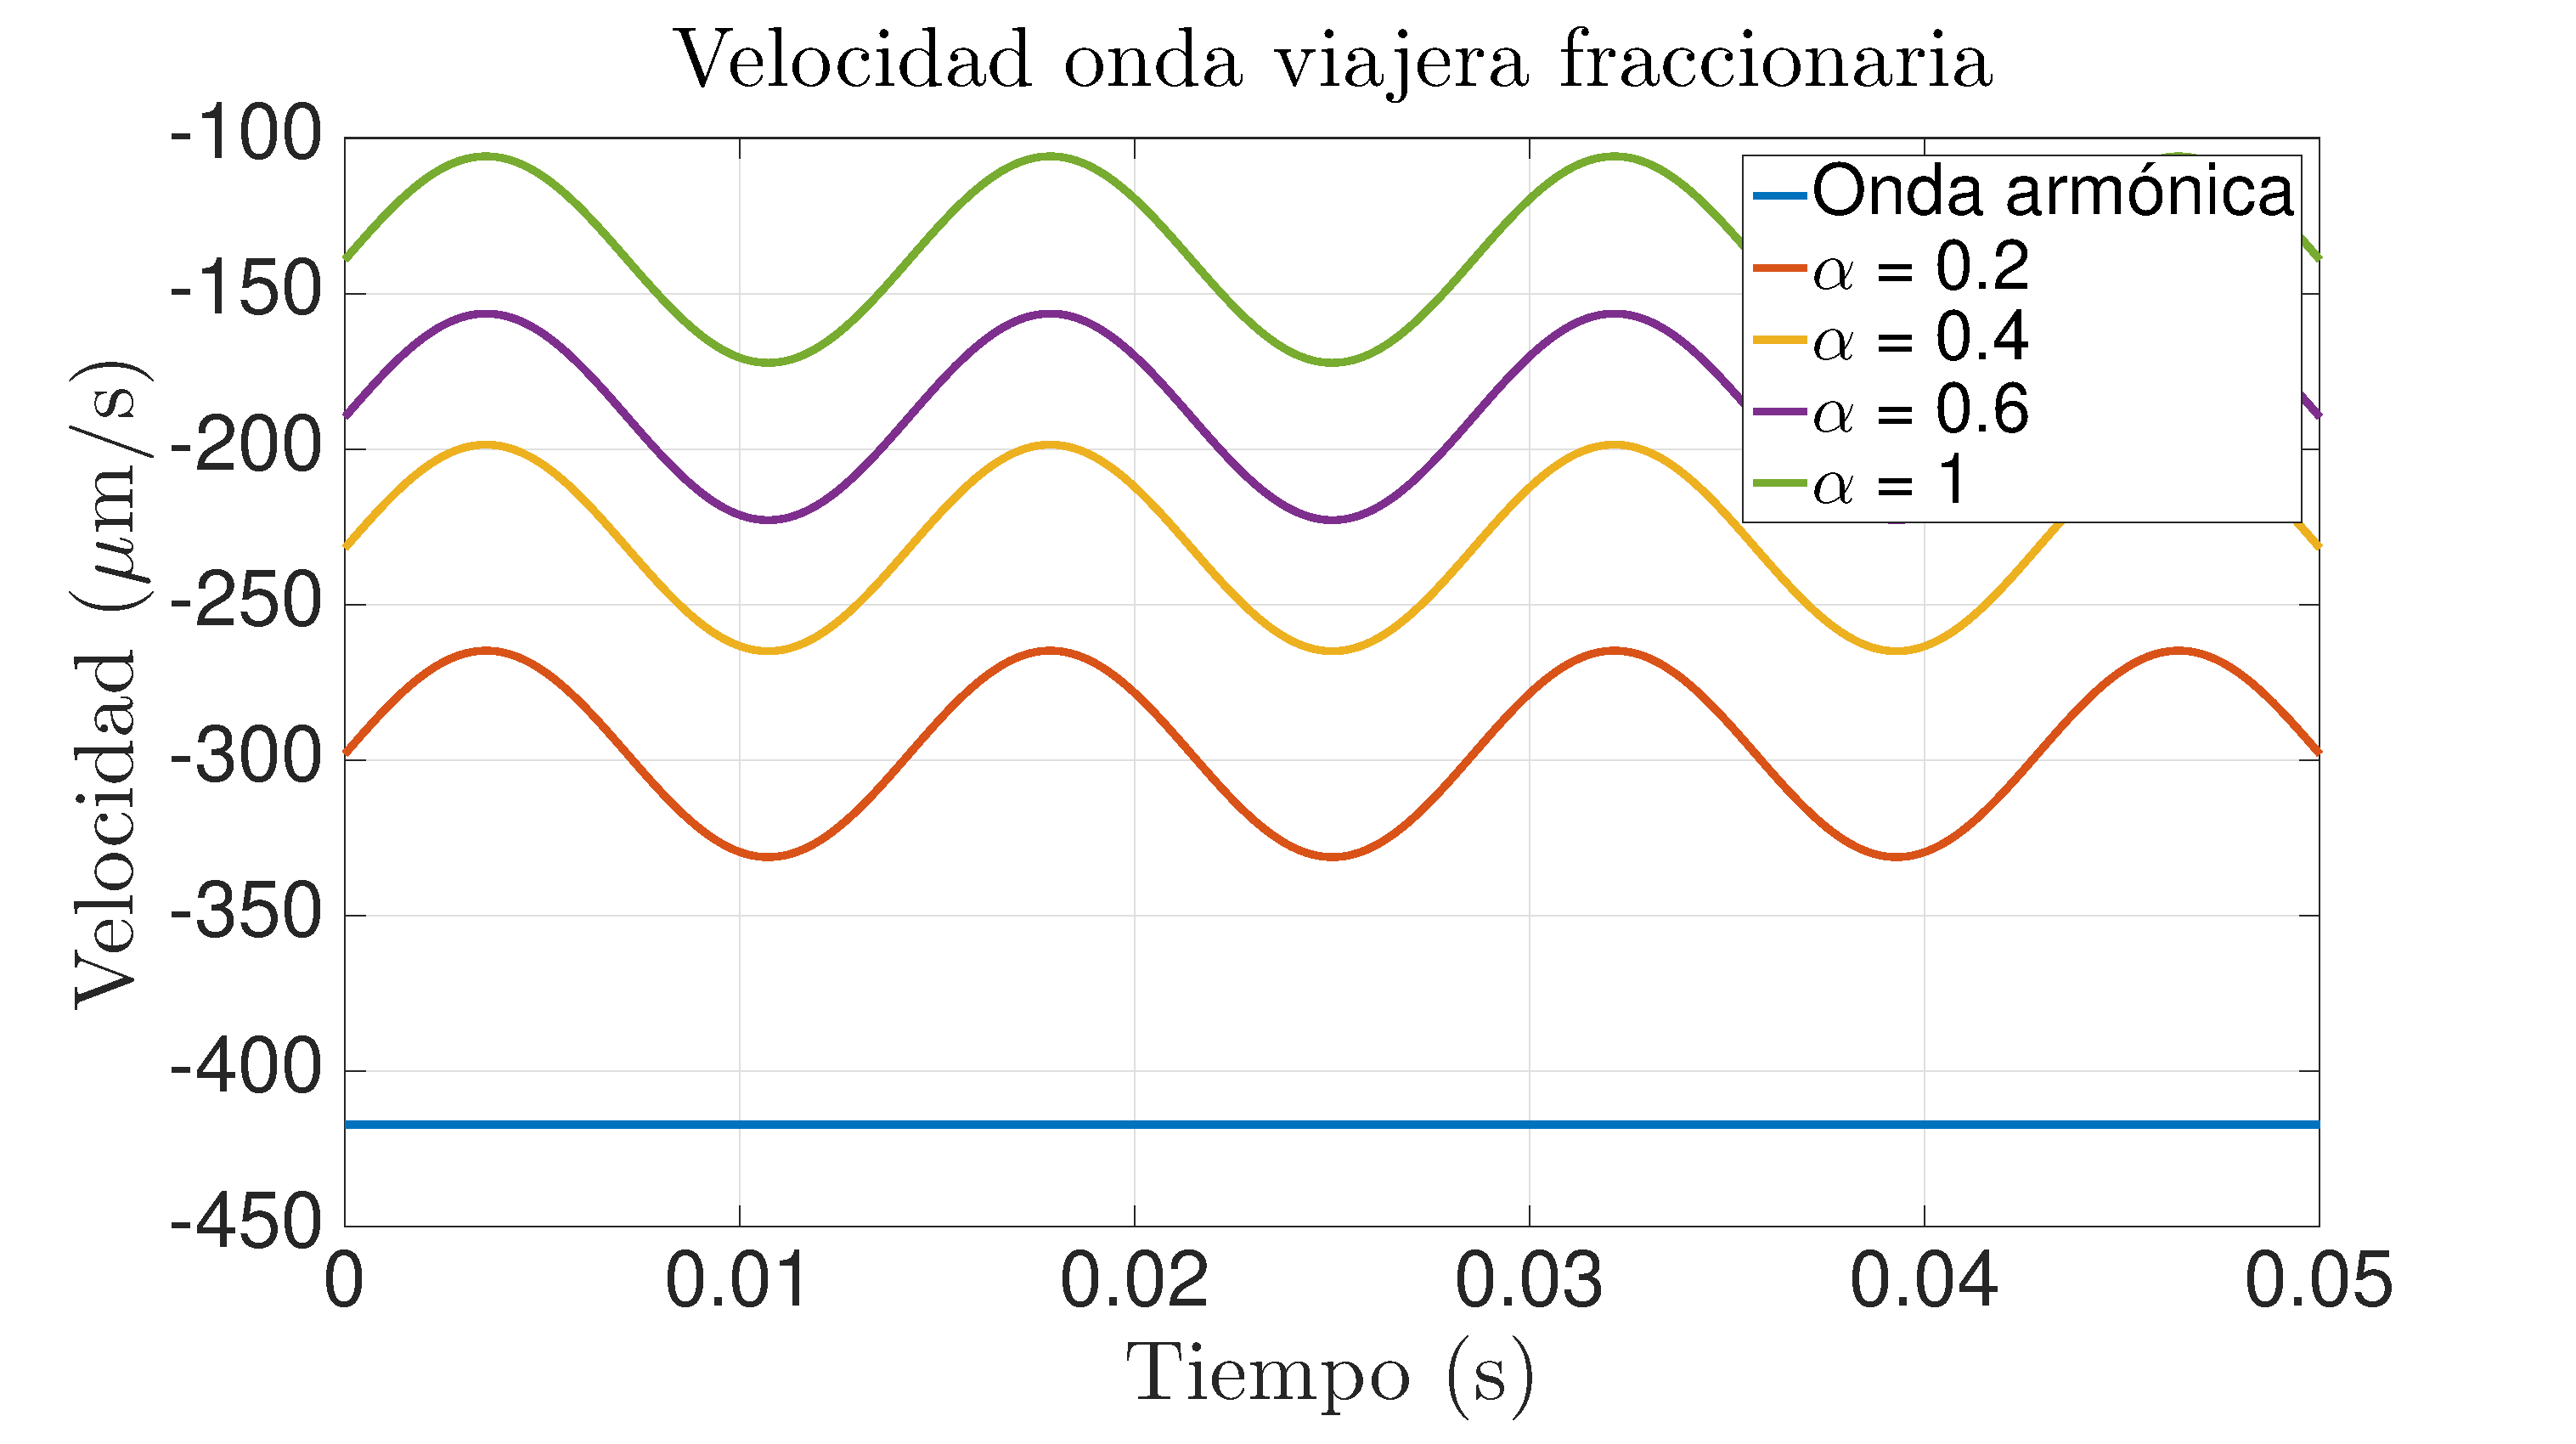
\includegraphics[width=0.85\textwidth]{Figuras/VCF}
  	\caption{Velocidad de avance onda viajera fraccionaria de pequeña señal.}
  	\label{fig:VCF}
\end{figure}

Los resultados obtenidos permite validar los afirmaciones realizadas anteriormente, es decir, la expresión de onda viajera fraccionaria proporciona una mayor fuerza de propulsión y por lo tanto velocidad de avance, ya que describe un crecimiento más rápido de las oscilaciones hasta alcanzar la amplitud máxima. Así mismo, coeficientes más bajos implican una mayor velocidad de avance, como se puede observar en la Figura, alcanzado 71.43\% de la velocidad óptima para un $\alpha$ = 0.2, en comparación al 33.33\% o 39.25\% alcanzado con la expresión \ref{eq:flag_fish_traveling_wave} con coeficiente lineal y posterior modulación, respectivamente.





















%---------------------------------------
% Capítulo 3: VELOCIDAD DE AVANCE DE ONDAS DE GRAN AMPLITUD
%---------------------------------------
% Resolución del problema a grandes dimensiones.
%---------------------------------------
\section{VELOCIDAD DE AVANCE DE ONDAS DE GRAN AMPLITUD} \label{sec:velocidad_grande}
%---------------------------------------
En la sección anterior se ha calculado la velocidad de avance generada para diferentes ondas viajeras bajo la suposición de oscilaciones muy pequeñas. Sin embargo, si la longitud del flagelo es considerablemente mayor que la longitud de onda y la sección de un diferencial de flagelo varía durante el desplazamiento transversal, no es posible aceptar la suposición realizada anteriormente ($ds \approx dx$) \cite{Gray1955}, y por lo tanto el diferencial de superficie ($ds$) se define por medio de la siguiente expresión
\begin{eqnarray}
	\label{eq:ds_big}
	ds = \sqrt{ 1 +\left(\frac{dy}{dx} \right)^2 } dx .
\end{eqnarray}

Además la expresión (\ref{eq:Vx_dx}) debe ser reformulada a partir las ecuaciones  (\ref{eq:dF_ds}), (\ref{eq:dF=}) y (\ref{eq:ds_big}) obteniendo que la velocidad de avance ahora se encuentra definida por: 
\begin{eqnarray}
\label{eq:Vx_dx}
	V_x (t) = \displaystyle  \frac{ (C_N - C_L) \displaystyle     \int_{0}^{\lambda}   \frac{ \frac{dy}{dt} \frac{dy}{dx} } { \sqrt{1 + \left( \frac{dy}{dx}\right)^2 } }  dx }
	{ \displaystyle  \frac{6 \pi R \mu}{n} +
	 \displaystyle   \int_{0}^{\lambda} {
		 \frac{C_L + C_N \left( \frac{dy}{dx} \right)^2}
	 			 { \sqrt{1 + \left( \frac{dy}{dx}\right)^2 } } } dx
	}
\end{eqnarray}

%---------------------------------------
\subsection{Descripción del script de integración numérica} \label{sec:descripcion_script2}
%-------------------------------------
Como consecuencia del cambio de la expresión que determina la velocidad de avance, se hace necesario modificar la función definida anteriormente para calcular la velocidad. Siendo reescrita como se muestra a continuación:
\begin{lstlisting}[]
	%% Calculo de la velocidad de avance por integración numérica.
    % Sea A = (dy/dx)^2
    
    % Vx =  (CN - CL) / sqrt(1 + A) * dy_dt * dy_dx dx 
    %       / ( Cc/n +  (CL + CN* A)  dx/ sqrt(1 + A) )

    for i=1:length(t);

      dy_dt =@(x) -(2*pi*Vp/lambda) * (c0 + c1.*x.^alfa  + c2.*x.^2)...
                  .* cos( (2*pi/lambda) * (x - Vp*t(i)) );
      
      dy_dx1 =@(x) (2*pi/lambda) .* (c0 + c1.*x.^alfa + c2.*x.^2)...
                   .* cos( (2*pi/lambda) * (x - Vp.*t(i)) );
      
      dy_dx2 =@(x) (2*c2.*x + alfa.*c1.*x.^(alfa-1))...
                   .* sin( (2*pi/lambda) * (x - Vp.*t(i)) ); 

      A = @(x) (dy_dx1(x) + dy_dx2(x)) .* (dy_dx1(x) + dy_dx2(x));

      vx_dx_num =@(x) ( (CN - CL) ./ sqrt(1 + A(x) ) )...
                      .*  dy_dt(x) .* ( dy_dx1(x) + dy_dx2(x));
                  
      vx_dx_dem =@(x)  ( CL + CN * A(x) ) ./ sqrt( 1 + A(x) ) ;
  

      % Función de integración numérica -- quadgk
      % Numerically evaluate integral, adaptive Gauss-Kronrod quadrature.
      int_num = quadgk(vx_dx_num,0,lambda);
      int_dem = quadgk(vx_dx_dem,0,lambda);

      Vx = [ Vx int_num / ( Cc/n + int_dem )];
    end

\end{lstlisting}

%---------------------------------------
\subsection{Cálculo y análisis de velocidad de onda viajera fraccionaria} \label{sec:analisis_velocidad2}
%-------------------------------------
Finalmente, se calcula las velocidades correspondiente a la ondas viajeras descritas en las Figuras \ref{fig:VCF} y \ref{fig:OVV}, cuyas magnitudes se encuentran representadas en la Figura \ref{fig:VCFB}.
\begin{figure}[!h] %  figure placement: here, top, bottom, or page
	\vspace*{3mm}
    \centering
    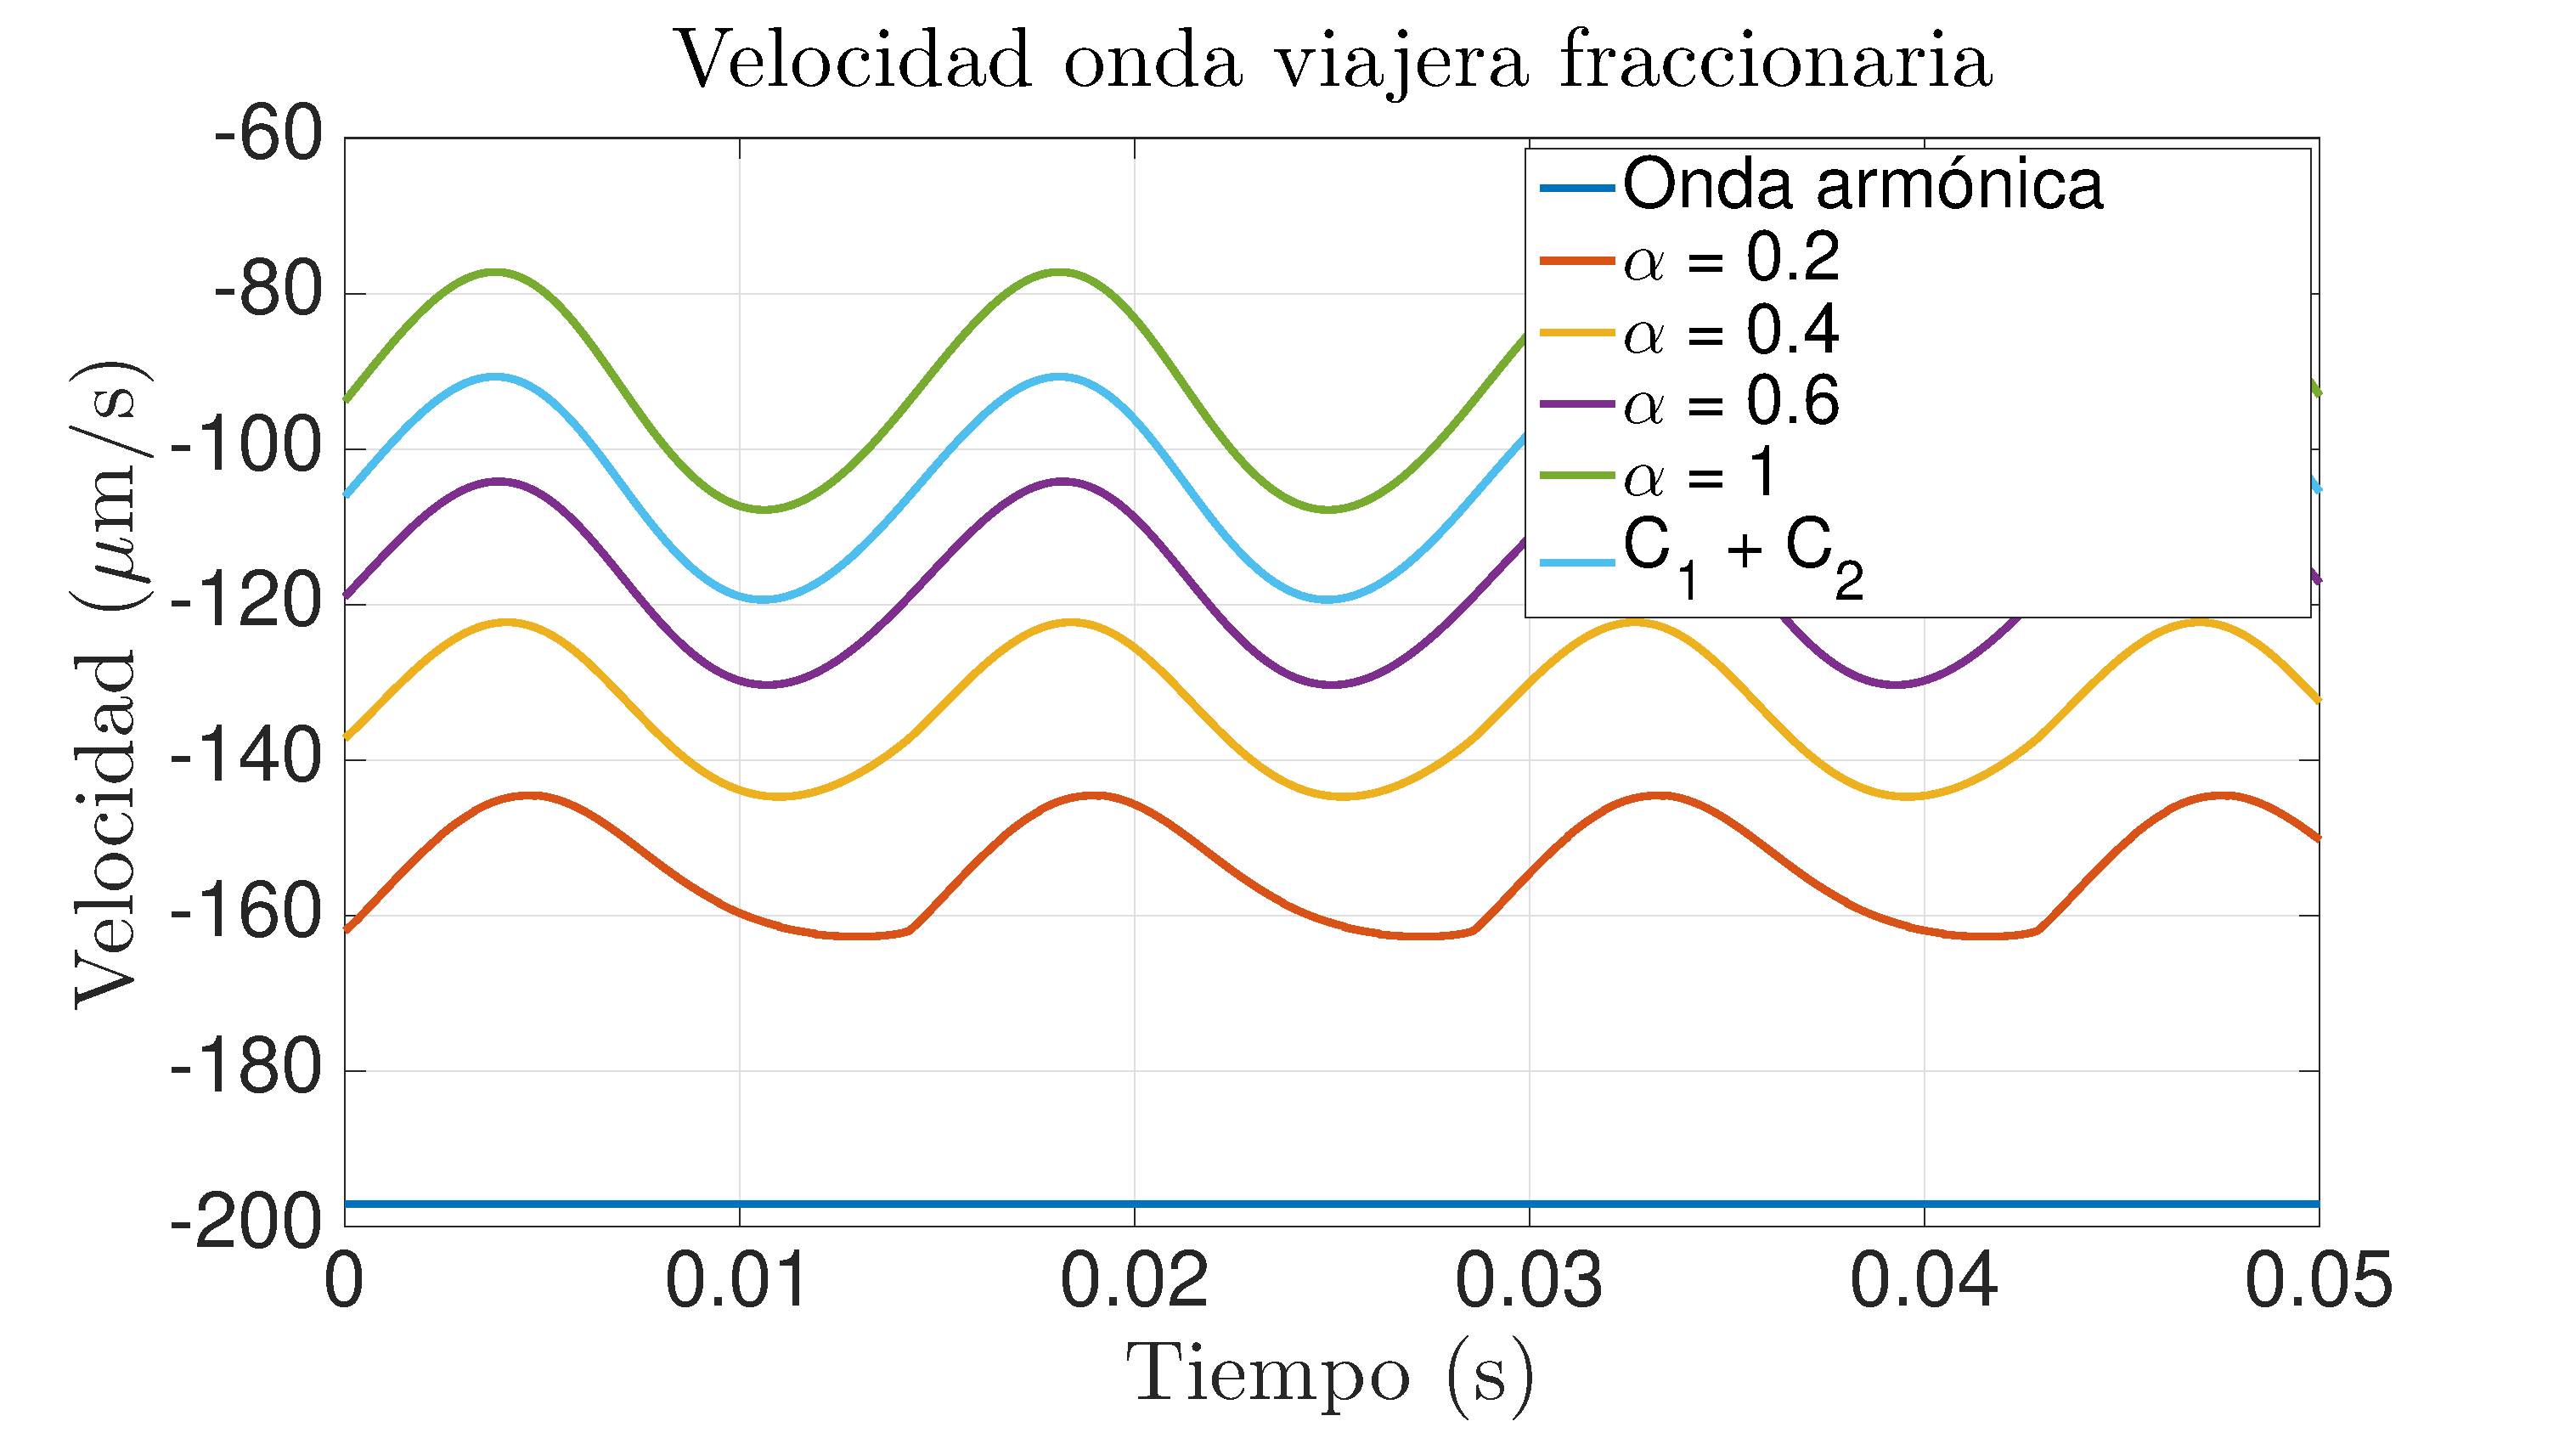
\includegraphics[width=0.85\textwidth]{Figuras/VCFB}
  	\caption{Velocidad de avance onda viajera fraccionaria de gran señal.}
  	\label{fig:VCFB}
\end{figure}

Nuevamente los resultados demuestra que la nueva expresión de onda viajera descrita proporciona una mayor velocidad de avance, aunque en esta ocasión se obtiene magnitudes menores, como consecuencia de emplear una ecuación más precisa sin el empleo de aproximaciones que simplifiquen el cálculo. Logrando un 82.23\% para un $\alpha$ = 0.2, 47.21\% y 53.81\% para el coeficiente de amplitud lineal y modulación, respectivamente.\\

También cabe destacar que la pérdida del carácter sinusoidal de la velocidad conforme disminuye el valor del parámetro $\alpha$, tal y como se muestra en la siguiente Figura \ref{fig:VCFB2}. Esto es debido a que la forma de onda cada vez alcanza una forma mas cercana a la onda armónica.
\begin{figure}[!h] %  figure placement: here, top, bottom, or page
	\vspace*{3mm}
    \centering
    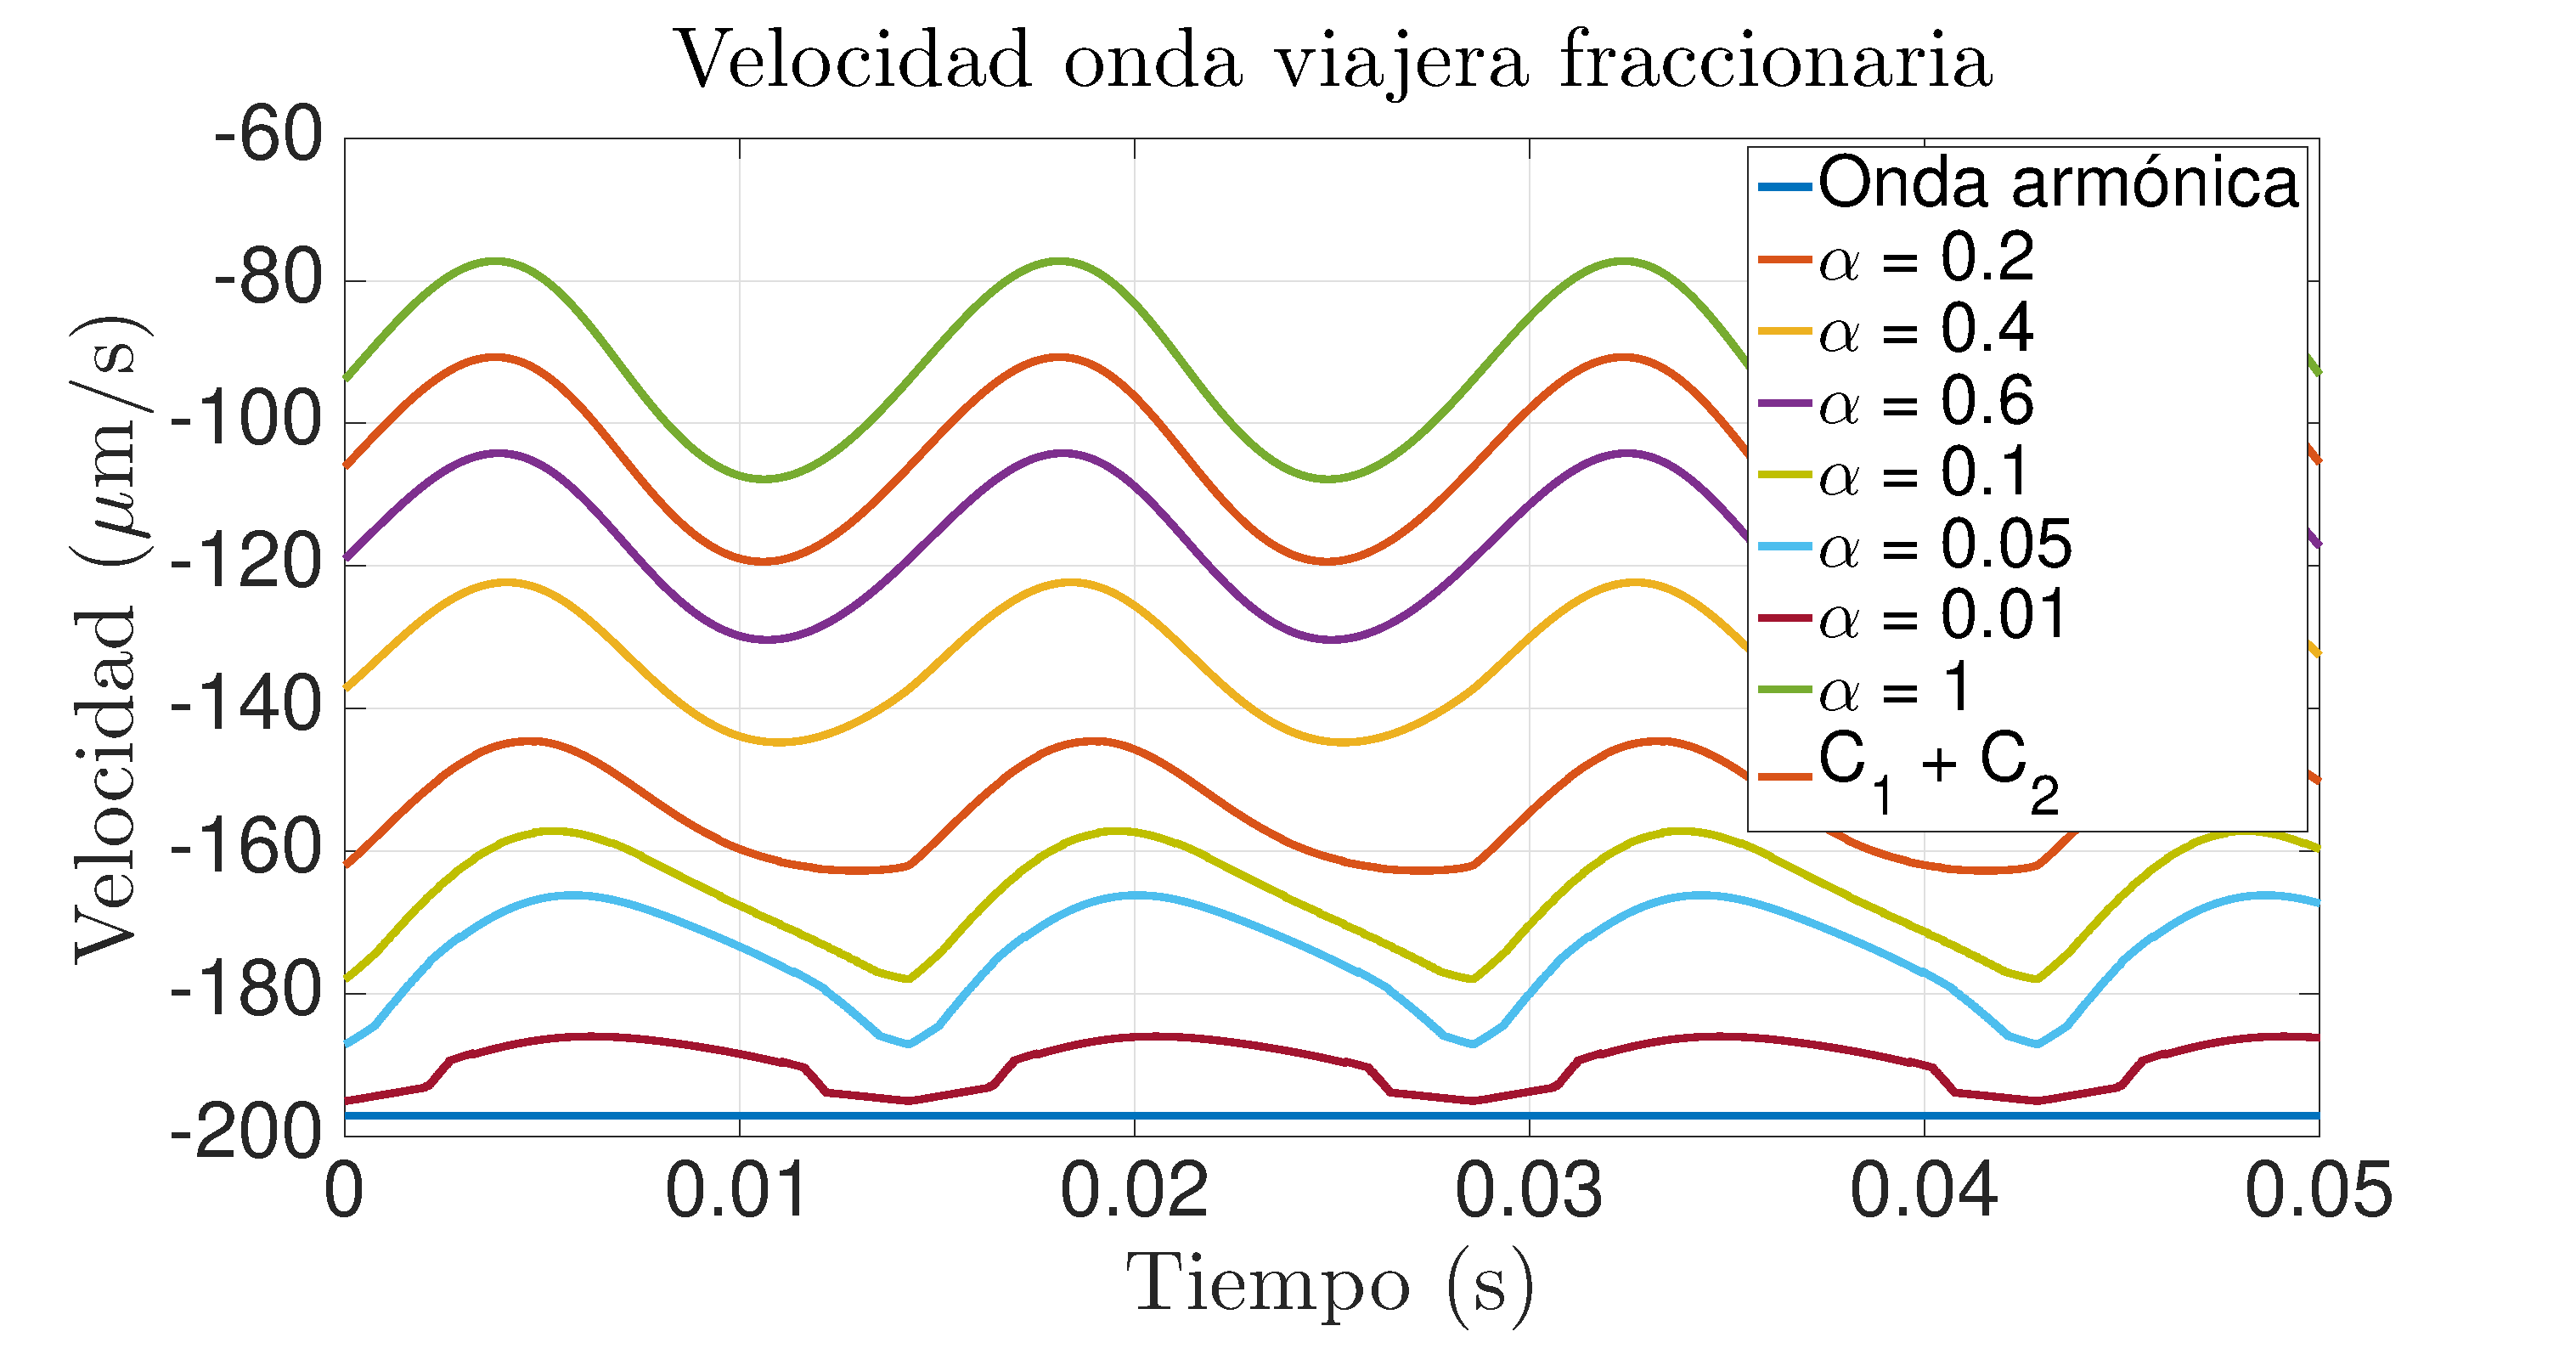
\includegraphics[width=0.85\textwidth]{Figuras/VCFB2}
  	\caption{Velocidad de avance onda viajera fraccionaria para valores bajos de $\alpha$.}
  	\label{fig:VCFB2}
\end{figure}
característica que no es tan evidente en el análisis anterior, ya que son necesario valores muy cercanos a cero para notar dicha característica.





%---------------------------------------
% Capítulo 4: CONCLUSIONES
%---------------------------------------
% Análisis de los resultados obtenidos.
%---------------------------------------
\section{CONCLUSIONES} \label{sec:conclusiones}
%---------------------------------------
El presente informe pone de manifiesto una nueva expresión de movimiento de onda viajera, el cual permite regular el crecimiento y modulación de la amplitud de las oscilaciones con un único parámetro, frente a las expresiones clásicas que requieren la combinación de varios parámetros para alcanzar los mismos objetivos. Además presenta las funciones necesarias para calcular mediante integración numérica la velocidad de avance lograda por este nueva expresión y las ya conocidas.\\

Respecto a los resultados extraídos del presente documento, permiten afirmar que el movimiento de onda viajera fraccionaria es más óptimo desde el punto de vista de la fuerza de propulsión y con ello la velocidad de avance, respecto a las otros tipos de movimientos indicados. Pues como han demostrado los resultados, la onda viajera fraccionaria presenta un mayor crecimiento de las oscilaciones y al mismo tiempo realiza una mejor modulación de las mismas, lo cual permite alcanzar un 70\% de la amplitud final en tan solo un 20\% de la distancia a la que se logra la amplitud máxima, frente a un 21\% de una onda viajera con crecimiento lineal. Por otro lado, en la velocidad de avance se alcanza el 82\% de la velocidad ideal que se conseguiría con un movimiento armónico, en comparación al 47\% de la onda de crecimiento lineal. Así mismo, la comparación de los resultados proporcionados por la onda viajera fraccionaria respecto a los obtenidos por la onda de crecimiento modulado, permite afirmar que dicho movimiento describe un movimiento mas óptimo y eficiente, ya que esta última únicamente lograr incrementar varias unidades los rendimientos correspondientes a la onda viajera de crecimiento lineal.\\

Finalmente, es posible afirmar que la expresión de onda viajera fraccionaria indicada ofrece un movimiento de propulsión más óptimo, lo cual se traduce a su vez una mayor fuerza de propulsión y velocidad de avance.


%--------------- CUERPO DEL DOCUMENTO ----------------


%---------------------------
% BIBLIOGRAFÍA
% ---


%%%%%%%%%%%%%%%%
\renewcommand{\refname}{\thesection \ \ REFERENCIAS}	% Título en el Header de la sección BIBLIOGRAFÍA.
\section{REFERENCIAS}
%	\nocite{*} 			% Comando para compilar las referencias cuando no se han realizado referencias a estas.
%%%%%%%%%%%%%%%%


%---
\renewcommand{\bibname}{}
\bibliographystyle{IEEEtran}
\bibliography{All_bib.bib}
%---------------------------


%--------------- ANEXOS ----------------

%%%%%%%%%%%%%%%%% 
\newpage
\appendix
\addappheadtotoc
%\appendixpage
%%%%%%%%%%%%%%%%%

%---------------------------------------
% Portada Anexos
\newcounter {pageAnexo}
\setcounter{pageAnexo}{\thepage}
\stepcounter{pageAnexo}
%%%%%%%%%%%%%%%%%%%% Porrtada.tex %%%%%%%%%%%%%%%%%%%%%%%%%%%%%%%%%%%%%%%%%%%%%%%%
% LaTeX Template for UEx - EII documents
% José Emilio Traver Becerra & David Palomeque Mangut
% Use at your own risk, send complaints to {jotraverb,dpalomeq}@alumnos.unex.es
%%%%%%%%%%%%%%%%%%%%%%%%%%%%%%%%%%%%%%%%%%%%%%%%%%%%%%%%%%%%%%%%%%%%%%%%%%%%%%%%
\begin{titlepage}
\begin{center}
\begin{LARGE}
\textbf{Universidad de Extremadura} \\
\end{LARGE}
\ \\
\begin{Large}
Escuela de Ingenierías Industriales\\
\end{Large}
\ \\
\begin{large}
\Asignatura
\end{large}
\end{center}
\vspace{6cm}
\begin{flushright}
\begin{huge}
%\begin{large}
\textbf{ANEXOS}
%\end{large}
\end{huge}
\end{flushright}
\vspace{10cm}
\begin{center}
Traver Becerra, José Emilio \\
\Degree
\end{center}
	\begin{center}
		\textbf{\myLocation, \myTime}
	\end{center}
\end{titlepage}


\setcounter{page}{\thepageAnexo}	
%---------------------------------------

%---------------------------------------
% Anexo 1: CÁLCULO DE LA VELOCIDAD PARA ONDAS PEQUEÑAS
%---------------------------------------	
%---------------------------------------
\section{CÁLCULO DE LA VELOCIDAD PARA ONDAS PEQUEÑAS} \label{anex:Anexo1}
%---------------------------------------
A continuación se muestra la función desarrollada para el cálculo de la velocidad de avance cuando se supone que las oscilaciones son pequeñas y la longitud de onda es similar a la longitud el flagelo.

\begin{lstlisting}[]
function [ NVx, TVx, t] = vxs(c0,c1,c2,alfa,teorico,Tf,Ts)
%VXS Calcula la velocidad de avance generada por una onda viajera del
%   tipo y = (c0 + c1*x^alfa + c2*x^2) * sin((2*pi/lambda)*(x-Vp*t)), bajo
%   las condiciones de oscilaciones de pequeña señal.
%
%   [NVx, TVx, T] = vxs(c0,c1,c2,alfa), NVx, es la velocidad generada por el
%   movimiento anterior con los coeficientes indicados, calculada mediante
%   integración numérica. TVx es la velocidad de propulsión calculada de
%   mediante la expresión algebraica, únicamente es calculada cuando el 
%   parametro teorico es verdadero. T denota el vector de tiempo.
%
%   'Teorico', valor boleano que permite calcular la velocidad mediante su
%   expresión algebraica. Únicamente válido para alfa = 1.
%
%   'Tf', indica el tiempo máximo de vector de tiempo T, que será devuelto.
%
%   'Ts', indica el paso de muestro del vector de tiempo.
%
%   Ejemplo:
%       Calcular el valor numérico y téorico.
%       [ NVC0, TVC0,T] = vxs(4e-6,0,0,1,1);
%
%   Ejemplo:
%       Calcular el valor numérico.
%       [ NVC1, TVC1,T] = vxs(0,4/24,0,1,0);
%
%   Ejemplo:
%       Calcular velocidad onda viajera fraccionaria.
%       [ NVF0,~,T] = vxs(0,4e-6/24e-6^.2,0,0.2,0);
%
%   Ejemplo:
%       Calcular velocidad para diferentes tiempos.
%       [ NVF0,~,T] = vxs(0,4/3*4/24,-4e-6/(3*24e-6^2),1,0,5e-2,1e-5);
%
%   
%   See also QUADGK.

    % -----------------------------
    % Parametros de Simulación
    % -----------------------------
    if (nargin < 5)
        Ts = 1e-5;      % Tiempo de Muestro
        Tf = 5e-2;      % Tiempo de Simulación
        teorico = 0;
    elseif (nargin < 6)
        Ts = 1e-5;      % Tiempo de Muestro
        Tf = 5e-2;      % Tiempo de Simulación    
    elseif (nargin < 7)
        Ts = 1e-5;      % Tiempo de Muestro    
    end

    t = 0:Ts:Tf;        % Vector de tiempo.
    NVx = [];

    % -----------------------------
    % Valores de la ecuación diferencial
    % -----------------------------

    mu = 7e-4;        % Viscosidad del medio. Fuente: Simulation of Swimming
                      %     Nanorobots in Biological Fluids (ieenano)
    f=35;             % Frecuencia de propagación.
    lambda = 24e-6;   % Longitud de onda de la onda viajera.
    n = 3;            % Numero de ondas simultaneas en el flagelo.      
    Vp = lambda * f;  % Velocidad de propagación de la onda viajera.
    R = 0.5e-6;       % Radio de la cabeza 
    d = 0.2e-6;       % Radio del flagelo
    L = n*lambda;     % Longitud del flagelo

    % Se puede calcular mirar ABF 
    % THE PROPULSION OF SEA-URCHIN SPERMATOZOA BY J. GRAY* AND G. J. 
    CL = - (2*pi*mu)/(log(d/(2*lambda))+(1/2));  
    CN = 2*CL;

    Cc = 6*pi*mu*R;          % Coeficiente de arrastre de la cabeza

    %% Calculo de la velocidad de avance por integración teórica.
    % Solo válida para teorico = 1

    if (teorico == 1)
        
        TVx = pi * f * ((CN - CL)/CL) *...
            ( 1/ (1 + (6 * pi * mu * R)/(n * lambda * CL) ) )...
            * ( -2*pi*c0^2/lambda - 2*pi*c0*c1 - (4*pi*lambda*c0*c2)/3 ...
            + c0*c1*sin(4*pi*f*t) + c0*c2*sin(4*pi*f*t)...
            - 2*pi*lambda*c1^2/3 - pi*lambda^2*c1*c2...
            + (lambda*c1^2/2)*sin(4*pi*f*t) + (lambda^2)*c1*c2*sin(4*pi*f*t)...
            - (2*pi*lambda^3*c2^2)/5 + (lambda^3*c2^2/2)*sin(4*pi*f*t) );
    else
        TVx = 0;
    end

    %% Calculo de la velocidad de avance por integración numérica.

    % Vx = (n * (CN - CL)) / (Cc + n * lambda * CL) * ( dy / dt * dy/dx dx)
    % Vx = |------------- vx_coeff ---------------| * |------ vx_dx -------|
    %                                         |-- dy_dt * (dy_dx1 + dy_dx2) --|

    vx_coeff = (  (1/lambda) * (CN - CL) / CL )...
                * ( 1 / (1 + Cc/ ( n * lambda * CL) ) ) ;

    for i=1:length(t);

        dy_dt =@(x) -(2*pi*Vp/lambda) * (c0 + c1.*x.^alfa  + c2.*x.^2)...
                    .* cos( (2*pi/lambda) * (x - Vp*t(i)) );

        dy_dx1 =@(x) (2*pi/lambda) .* (c0 + c1.*x.^alfa + c2.*x.^2)...
                    .* cos( (2*pi/lambda) * (x - Vp.*t(i)) );

        dy_dx2 =@(x) (2*c2.*x + alfa.*c1.*x.^(alfa-1))...
                    .* sin( (2*pi/lambda) * (x - Vp.*t(i)) ); 

        vx_dx =@(x) dy_dt(x) .* (dy_dx1(x) + dy_dx2(x));                                     

        % Función de integración numérica -- quadgk
        % Numerically evaluate integral, adaptive Gauss-Kronrod quadrature.
        NVx = [NVx  quadgk(vx_dx,0,lambda)];
    end

    NVx = NVx .* vx_coeff;
    
end
\end{lstlisting}


%---------------------------------------
% Anexo 2: REPRESENTACIÓN DE RESULTADOS DE ONDA PEQUEÑA
%---------------------------------------	
%---------------------------------------
\section{REPRESENTACIÓN DE RESULTADOS DE ONDA PEQUEÑA} \label{anex:Anexo2}
%---------------------------------------
A continuación se muestra el script desarrollado para la representación y cálculo de la velocidad de avance cuando se supone que las oscilaciones son pequeñas y los términos de segundo orden pueden ser obviados.

\begin{lstlisting}[]
%% VERIFICACIÓN Y ANÁLISIS VXS
% Este script realiza la representación de diferentes tipos de ondas
% viajeras, y calcula la velocidad de avance generada por cada una de
% ellas. Realizando posteriormente una gráfica de comparativa de
% velocidades.
% Cálculos realizados en este script atiendes nas consideraciones de onda
% de pequeña amplitud.

%% Representación movimiento de onda viajera clasico
figure(1)
print_traveling_wave(4e-6,0,0,1,[  0    0.4470    0.7410]);
hold on

print_traveling_wave(0,4/24,0,1,[0.4660    0.6740    0.1880]);

% Para C1 y C2, n y m son multiplos de la longitud de onda.  

% C1 = (A / (n*lambda) ) + ( m / (m - n) ) 
%    * (A / (m * lambda) - n * A / (m * lambda) )

% C2 = ( m / (m - n) ) * (A / ( n * m * lambda^2) - A / (m * lambda^2) )

% Para n = 1 y m = 3
print_traveling_wave(0,4/3*4/24,-4e-6/(3*24e-6^2),1,[0.6350,0.0780,0.1840]);

% Para n = 1 y m = 2
%print_traveling_wave(0,3/2*4/24,-4e-6/(2*24e-6^2),1,[0.6350,0.0780,0.1840]);
hold off

%% Representación movimiento de onda viajera fraccionario
figure(2)
print_traveling_wave(4e-6,0,0,1,[  0    0.4470    0.7410]);
hold on
print_traveling_wave(0,4e-6/24e-6^.2,0,0.2,[0.8500    0.3250    0.0980]);
print_traveling_wave(0,4e-6/24e-6^.4,0,0.4,[0.9290    0.6940    0.1250]);
print_traveling_wave(0,4e-6/24e-6^.6,0,0.6,[0.4940    0.1840    0.5560]);
print_traveling_wave(0,4/24,0,1,[0.4660    0.6740    0.1880]);
hold off


%% Verificación y validación del algoritmo de integración numérica.
clear all;
% Vector de tiempo
t = [];

% Cálculo velocidad de avance
[ NVC0, TVC0,t] = vxs(4e-6,0,0,1,1);
[ NVC1, TVC1,~] = vxs(0,4/24,0,1,1);
[ NVC2, TVC2,t] = vxs(0,4/3*4/24,-4e-6/(3*24e-6^2),1,1);
[ NVF0,~,~] = vxs(0,4e-6/24e-6^.2,0,0.2,0);
[ NVF1,~,~] = vxs(0,4e-6/24e-6^.4,0,0.4,0);
[ NVF2,~,~] = vxs(0,4e-6/24e-6^.6,0,0.6,0);


%% Representación de los resultados de velocidad
% Comparación de velocidades para C0
figure(3)
subplot(211)
plot(t,TVC0.*1e6,'Linewidth',4)
hold on
plot(t,NVC0.*1e6,'--r','Linewidth',4);
hold off
grid
ylabel('Velocidad ($\mu$m/s)','Interpreter','latex','FontSize',40)
title('Velocidad de avance para c$_0$','Interpreter','latex','FontSize',44)
tiy=get(gca,'ytick')';
set(gca, 'fontsize', 44,'yticklabel',num2str(tiy,'%.2f'));
legend('Valor Teórico','Valor Numérico');

subplot(212)
% RMSE
plot(t,sqrt(((NVC0 - TVC0).^2)./length(TVC0)).*1e2,'Linewidth',1)
grid
ylabel('RMSE (\%)','Interpreter','latex','FontSize',40)
xlabel('Tiempo (s)','Interpreter','latex','FontSize',40)
set(gca, 'fontsize', 44);

% Comparación de velocidades para C1
figure(4)
subplot(211)
plot(t,TVC1.*1e6,'Linewidth',4)
hold on
plot(t,NVC1.*1e6,'--r','Linewidth',4);
hold off
grid
ylabel('Velocidad ($\mu$m/s)','Interpreter','latex','FontSize',40)
title('Velocidad de avance para c$_1$','Interpreter','latex','FontSize',44)
set(gca, 'fontsize', 44);
legend('Valor Teórico','Valor Numérico');

subplot(212)
% RMSE
plot(t,sqrt(((NVC1 - TVC1).^2)./length(TVC1)).*1e2,'Linewidth',1)
grid
ylabel('RMSE (\%)','Interpreter','latex','FontSize',40)
xlabel('Tiempo (s)','Interpreter','latex','FontSize',40)
set(gca, 'fontsize', 44);


% Comparación de velocidades para C2
figure(5)
subplot(211)
plot(t,TVC2.*1e6,'Linewidth',4)
hold on
plot(t,NVC2.*1e6,'--r','Linewidth',4);
hold off
grid
ylabel('Velocidad ($\mu$m/s)','Interpreter','latex','FontSize',40)
title('Velocidad de avance para c$_1$ + c$_2$',...
        'Interpreter','latex','FontSize',44)
set(gca, 'fontsize', 44);
legend('Valor Teórico','Valor Numérico');

subplot(212)
% RMSE
plot(t,sqrt(((NVC2 - TVC2).^2)./length(TVC2)).*1e2)
grid
ylabel('RMSE (\%)','Interpreter','latex','FontSize',40)
xlabel('Tiempo (s)','Interpreter','latex','FontSize',40)
set(gca, 'fontsize', 44);


%% Representación de ñps resultados de velocidad de onda fraccionaria
figure(6)
plot(t,NVC0.*1e6,'Linewidth',4)
hold on
plot(t,NVF0.*1e6,'Linewidth',4);
plot(t,NVF1.*1e6,'Linewidth',4);
plot(t,NVF2.*1e6,'Linewidth',4);
plot(t,NVC1.*1e6,'Linewidth',4);
hold off
grid
ylabel('Velocidad ($\mu$m/s)','Interpreter','latex','FontSize',40)
xlabel('Tiempo (s)','Interpreter','latex','FontSize',40)
title('Velocidad onda viajera fraccionaria',...
        'Interpreter','latex','FontSize',44)
set(gca, 'fontsize', 44);
legend('Onda armónica','\alpha = 0.2','\alpha = 0.4',...
        '\alpha = 0.6','\alpha = 1');
\end{lstlisting}


%---------------------------------------
% Anexo 3: CÁLCULO DE LA VELOCIDAD PARA ONDAS DE GRAN AMPLITUD
%---------------------------------------	
%---------------------------------------
\section{CÁLCULO DE LA VELOCIDAD PARA ONDAS DE GRAN AMPLITUD} \label{anex:Anexo1}
%---------------------------------------
A continuación se muestra la función desarrollada para el cálculo de la velocidad de avance cuando se supone que las oscilaciones de gran amplitud.

\begin{lstlisting}[]
function [Vx, T] = vxb(c0,c1,c2,alfa,Tf,Ts)
%VXB Calcula la velocidad de avance generada por una onda viajera del
%   tipo y = (c0 + c1*x^alfa + c2*x^2) * sin((2*pi/lambda)*(x-Vp*t)), bajo
%   las condiciones de oscilaciones de gran señal.
%   [NVx, TVx, T] = vxs(c0,c1,c2,alfa), NVx, es la velocidad generada por el
%   movimiento anterior con los coeficientes indicados, calculada mediante
%   integración numérica. T denota el vector de tiempo.
%
%   'Tf', indica el tiempo máximo de vector de tiempo T, que será devuelto.
%
%   'Ts', indica el paso de muestro del vector de tiempo.
%
%   Ejemplo:
%       Calcular el valor numérico.
%       [ NVC0 T] = vxb(4e-6,0,0,1);
%
%   Ejemplo:
%       Calcular el valor numérico.
%       [ NVC1, T] = vxb(0,4/24,0,1);
%
%   Ejemplo:
%       Calcular velocidad onda viajera fraccionaria.
%       [ NVF0,T] = vxb(0,4e-6/24e-6^.2,0,0.2);
%
%   Ejemplo:
%       Calcular velocidad para diferentes tiempos.
%       [ NVF0,T] = vxb(0,4/3*4/24,-4e-6/(3*24e-6^2),1,5e-2,1e-5);
%
%   
%   See also QUADGK.

    % -----------------------------
    % Parametros de Simulación
    % -----------------------------
    if (nargin < 5)
        Ts = 1e-5;      % Tiempo de Muestro
        Tf = 5e-2;      % Tiempo de Simulación    
    elseif (nargin < 6)
        Ts = 1e-5;      % Tiempo de Muestro    
    end

    t = 0:Ts:Tf;        % Vector de tiempo.
    Vx = [];

    % -----------------------------
    % Valores de la ecuación diferencial
    % -----------------------------

    mu = 7e-4;        % Viscosidad del medio. Fuente: Simulation of Swimming
                      %     Nanorobots in Biological Fluids (ieenano)
    f=35;             % Frecuencia de propagación.
    lambda = 24e-6;   % Longitud de onda de la onda viajera.
    n = 3;            % Numero de ondas simultaneas en el flagelo.      
    Vp = lambda * f;  % Velocidad de propagación de la onda viajera.
    R = 0.5e-6;       % Radio de la cabeza 
    d = 0.2e-6;       % Radio del flagelo
    L = n*lambda;     % Longitud del flagelo

    % Se puede calcular mirar ABF 
    % THE PROPULSION OF SEA-URCHIN SPERMATOZOA BY J. GRAY* AND G. J. 
    CL = - (2*pi*mu)/(log(d/(2*lambda))+(1/2));  
    CN = 2*CL;

    Cc = 6*pi*mu*R;          % Coeficiente de arrastre de la cabeza

  
    %% Calculo de la velocidad de avance por integración numérica.
    % Sea A = (dy/dx)^2
    
    % Vx =  (CN - CL) / sqrt(1 + A) * dy_dt * dy_dx dx 
    %       / ( Ch/n +  (CL + CN* A) / sqrt(1 + A) )

    for i=1:length(t);

      dy_dt =@(x) -(2*pi*Vp/lambda) * (c0 + c1.*x.^alfa  + c2.*x.^2)...
                  .* cos( (2*pi/lambda) * (x - Vp*t(i)) );
      
      dy_dx1 =@(x) (2*pi/lambda) .* (c0 + c1.*x.^alfa + c2.*x.^2)...
                   .* cos( (2*pi/lambda) * (x - Vp.*t(i)) );
      
      dy_dx2 =@(x) (2*c2.*x + alfa.*c1.*x.^(alfa-1))...
                   .* sin( (2*pi/lambda) * (x - Vp.*t(i)) ); 

      A = @(x) (dy_dx1(x) + dy_dx2(x)) .* (dy_dx1(x) + dy_dx2(x));

      vx_dx_num =@(x) ( (CN - CL) ./ sqrt(1 + A(x) ) )...
                      .*  dy_dt(x) .* ( dy_dx1(x) + dy_dx2(x));
                  
      vx_dx_dem =@(x)  ( CL + CN * A(x) ) ./ sqrt( 1 + A(x) ) ;
  

      % Función de integración numérica -- quadgk
      % Numerically evaluate integral, adaptive Gauss-Kronrod quadrature.
      int_num = quadgk(vx_dx_num,0,lambda);
      int_dem = quadgk(vx_dx_dem,0,lambda);

      Vx = [ Vx int_num / ( Cc/n + int_dem )];
    end

    
end
\end{lstlisting}


%---------------------------------------
% Anexo 4: REPRESENTACIÓN RESULTADOS ONDA DE GRAN ONDA AMPLITUD
%---------------------------------------	
%---------------------------------------
\section{REPRESENTACIÓN RESULTADOS ONDA DE GRAN ONDA AMPLITUD} \label{anex:Anexo4}
%---------------------------------------
A continuación se muestra el script desarrollado para la representación y cálculo de la velocidad de avance cuando se supone que las oscilaciones de gran amplitud.

\begin{lstlisting}[]
%% ANÁLISIS VXB
% Este script realiza la representación de diferentes tipos de ondas
% viajeras, y calcula la velocidad de avance generada por cada una de
% ellas. Realizando posteriormente una gráfica de comparativa de
% velocidades.
% Cálculos realizados en este script atiendes nas consideraciones de onda
% de gran amplitud.

%% Representación movimiento de onda viajera analizados
figure(1)
print_traveling_wave(4e-6,0,0,1,[  0    0.4470    0.7410]);
hold on
print_traveling_wave(0,4/24,0,1,[0.4660    0.6740    0.1880]);

% Para C1 y C2, n y m son multiplos de la longitud de onda.  

% C1 = (A / (n*lambda) ) + ( m / (m - n) )
%    * (A / (m * lambda) - n * A / (m * lambda) )

% C2 = ( m / (m - n) ) * (A / ( n * m * lambda^2) - A / (m * lambda^2) )

% Para n = 1 y m = 3
print_traveling_wave(0,4/3*4/24,-4e-6/(3*24e-6^2),1,[0.6350,0.0780,0.1840]);

% Para n = 1 y m = 2
%print_traveling_wave(0,3/2*4/24,-4e-6/(2*24e-6^2),1,[0.6350,0.0780,0.1840]);

% Ondas viajeras fraccionarias
print_traveling_wave(0,4e-6/24e-6^.01,0,0.01,[0.6350    0.0780    0.1840]);
print_traveling_wave(0,4e-6/24e-6^.05,0,0.05,[0.3010    0.7450    0.9330]);
print_traveling_wave(0,4e-6/24e-6^.1,0,0.1,[0.7500    0.7500         0]);
print_traveling_wave(0,4e-6/24e-6^.2,0,0.2,[0.8500    0.3250    0.0980]);
print_traveling_wave(0,4e-6/24e-6^.4,0,0.4,[0.9290    0.6940    0.1250]);
print_traveling_wave(0,4e-6/24e-6^.6,0,0.6,[0.4940    0.1840    0.5560]);
hold off

%% Verificación y validación del algoritmo de integración numérica.
clear all;
% Vector de tiempo
t = [];
[ VC0,t] = vxb(4e-6,0,0,1);
[ VC1,~] = vxb(0,4/24,0,1);
[ VC2,~] = vxb(0,4/3*4/24,-4e-6/(3*24e-6^2),1);
[ VF0,~] = vxb(0,4e-6/24e-6^.2,0,0.2);
[ VF1,~] = vxb(0,4e-6/24e-6^.4,0,0.4);
[ VF2,~] = vxb(0,4e-6/24e-6^.6,0,0.6);
[ VF3,~] = vxb(0,4e-6/24e-6^.1,0,0.1);
[ VF4,~] = vxb(0,4e-6/24e-6^.05,0,0.05);
[ VF5,~] = vxb(0,4e-6/24e-6^.01,0,0.01);

%% Representación de los resultados de velocidad de onda fraccionaria
figure(6)
plot(t,VC0.*1e6,'Linewidth',4)
hold on
plot(t,VF0.*1e6,'Linewidth',4);
plot(t,VF1.*1e6,'Linewidth',4);
plot(t,VF2.*1e6,'Linewidth',4);
plot(t,VF3.*1e6,'Linewidth',4);
plot(t,VF4.*1e6,'Linewidth',4);
plot(t,VF5.*1e6,'Linewidth',4);
plot(t,VC1.*1e6,'Linewidth',4);
plot(t,VC2.*1e6,'Linewidth',4);
hold off
grid
ylabel('Velocidad ($\mu$m/s)','Interpreter','latex','FontSize',40)
xlabel('Tiempo (s)','Interpreter','latex','FontSize',40)
title('Velocidad onda viajera fraccionaria',...
        'Interpreter','latex','FontSize',44)
set(gca, 'fontsize', 44);
legend('Onda armónica','\alpha = 0.2','\alpha = 0.4','\alpha = 0.6',...
 '\alpha = 0.1','\alpha = 0.05','\alpha = 0.01','\alpha = 1','C_1 + C_2');
 \end{lstlisting}




%--------------- ANEXOS ----------------

% -------------------%
% -------------------%
\end{document}%------%
% -------------------%
% -------------------%